% =====================================================================
%  An Autonomous Mobile-Manipulation Stack for Greenhouse Strawberry
%  Harvesting: from a Webots Prototype to a ROS 2 / Gazebo Digital Twin
%
%  PFA (Projet de Fin d'Annee) technical report
%  Compile:  make        -> report.pdf     (pdflatex + bibtex + 2x pdflatex)
% =====================================================================
\documentclass[conference]{IEEEtran}

% =====================================================================
%  preamble.tex -- packages, styles and the flowchart visual language
%  Smart Agriculture Digital Twin -- KUKA YouBot -- PFA technical report
% =====================================================================
%
%  Everything that is not prose lives here so the section files stay
%  readable. Three things are defined below and used everywhere else:
%
%    1. IEEE-conformant typography (IEEEtran, Times, two columns).
%    2. A code-listing style per language (bash / python / xml / yaml).
%    3. THE FLOWCHART LANGUAGE: a fixed set of coloured node shapes and
%       three phase bands -- INITIALISATION, MAIN LOOP, TERMINATION --
%       so that every flowchart in this report reads the same way.
%
%  Compile with:  make        (see Makefile, uses pdflatex + bibtex)
% =====================================================================

% ------------------------------------------------------- encoding, fonts
\usepackage[T1]{fontenc}
\usepackage[utf8]{inputenc}
\usepackage[english]{babel}
\usepackage{textcomp}

% ------------------------------------------------------- maths
\usepackage{amsmath}
\usepackage{amssymb}
\usepackage{amsfonts}
\usepackage{bm}

% ------------------------------------------------------- tables & figures
\usepackage{graphicx}
\usepackage{booktabs}
\usepackage{array}
\usepackage{multirow}
\usepackage{tabularx}
\usepackage{longtable}
\usepackage{float}
\usepackage{caption}
\usepackage{subcaption}

% ------------------------------------------------------- code listings
\usepackage{listings}
\usepackage{xcolor}

% ------------------------------------------------------- pseudocode
\usepackage{algorithm}
\usepackage{algpseudocode}

% ------------------------------------------------------- drawings
\usepackage{tikz}
\usetikzlibrary{shapes.geometric,shapes.misc,shapes.symbols,arrows.meta,
                positioning,fit,backgrounds,calc,decorations.pathreplacing,
                patterns}

% ------------------------------------------------------- IEEE citations
\usepackage{cite}
\usepackage{url}

% ------------------------------------------------------- misc
\usepackage{enumitem}
\usepackage{ifthen}

% hyperref must come last
\usepackage[hidelinks,breaklinks=true]{hyperref}

% =====================================================================
%  1. COLOUR PALETTE
% =====================================================================
%  One palette for the whole document. The three phase colours are the
%  spine of every flowchart; the accent colours are for emphasis inside
%  tables and listings. Chosen to stay legible when printed in grey.
% ---------------------------------------------------------------------

% --- flowchart phase bands (light fills, saturated borders)
\definecolor{phaseInitFill}{HTML}{DCE9F7}   % blue   -- INITIALISATION
\definecolor{phaseInitLine}{HTML}{2E5F9E}
\definecolor{phaseMainFill}{HTML}{E2F3E4}   % green  -- MAIN LOOP
\definecolor{phaseMainLine}{HTML}{2E7D32}
\definecolor{phaseEndFill}{HTML}{FBE4DC}    % red    -- TERMINATION
\definecolor{phaseEndLine}{HTML}{C0392B}

% --- flowchart node fills
\definecolor{nodeTerm}{HTML}{FFD9A0}        % terminal  (start / stop)
\definecolor{nodeTermLine}{HTML}{B26B00}
\definecolor{nodeProc}{HTML}{FFFFFF}        % process
\definecolor{nodeProcLine}{HTML}{37474F}
\definecolor{nodeDec}{HTML}{FFF6C2}         % decision
\definecolor{nodeDecLine}{HTML}{B8860B}
\definecolor{nodeIO}{HTML}{DDE6FA}          % input / output (ROS topic)
\definecolor{nodeIOLine}{HTML}{3F51B5}
\definecolor{nodeSub}{HTML}{E8DAF5}         % subroutine / library call
\definecolor{nodeSubLine}{HTML}{6A1B9A}
\definecolor{nodeNote}{HTML}{F5F5F5}        % annotation
\definecolor{nodeFail}{HTML}{FADBD8}        % failure / recovery branch
\definecolor{nodeFailLine}{HTML}{922B21}

% --- semantic accents used in prose and tables
\definecolor{okGreen}{HTML}{1E7B34}
\definecolor{warnAmber}{HTML}{B7791F}
\definecolor{badRed}{HTML}{B03A2E}
\definecolor{codeGray}{HTML}{4F4F4F}
\definecolor{codeBg}{HTML}{F7F7F9}
\definecolor{codeKey}{HTML}{0B5394}
\definecolor{codeStr}{HTML}{A31515}
\definecolor{codeCom}{HTML}{5B7C5B}

% shorthand for verdict marks in SWOT and results tables
\newcommand{\ok}[1]{\textcolor{okGreen}{\textbf{#1}}}
\newcommand{\warn}[1]{\textcolor{warnAmber}{\textbf{#1}}}
\newcommand{\bad}[1]{\textcolor{badRed}{\textbf{#1}}}

% =====================================================================
%  2. CODE LISTINGS
% =====================================================================
%  Two columns are narrow, so listings default to \footnotesize and
%  break long lines with a visible arrow. Wide listings go in a
%  figure*/table* float instead of being shrunk further.
% ---------------------------------------------------------------------
\lstdefinestyle{base}{
  basicstyle       = \ttfamily\footnotesize\color{codeGray},
  keywordstyle     = \color{codeKey}\bfseries,
  stringstyle      = \color{codeStr},
  commentstyle     = \color{codeCom}\itshape,
  numberstyle      = \tiny\color{gray},
  backgroundcolor  = \color{codeBg},
  frame            = single,
  rulecolor        = \color{gray!40},
  framesep         = 3pt,
  xleftmargin      = 6pt,
  xrightmargin     = 2pt,
  breaklines       = true,
  breakatwhitespace= false,
  postbreak        = \mbox{\textcolor{gray}{$\hookrightarrow$}\space},
  showstringspaces = false,
  tabsize          = 2,
  columns          = fullflexible,
  keepspaces       = true,
  upquote          = true,
  captionpos       = b,
}
\lstdefinestyle{bash}{style=base,language=bash,
  morekeywords={ros2,colcon,source,export,sudo,apt,git,gz,rviz2,make}}
\lstdefinestyle{python}{style=base,language=Python}
\lstdefinestyle{xml}{style=base,language=XML,
  morestring=[b]",moredelim=[s][\color{codeKey}]{<}{>}}
\lstdefinestyle{yaml}{style=base,
  keywords={true,false,null},
  comment=[l]{\#},
  moredelim=[l][\color{codeKey}]{:},
}
\lstset{style=base}

% =====================================================================
%  3. THE FLOWCHART VISUAL LANGUAGE
% =====================================================================
%  Every flowchart in this report uses these shapes and only these.
%  The reader learns the alphabet once, in Fig. 1 (the legend), and can
%  then read every later diagram without a caption.
%
%  SHAPES (ISO 5807 / classic flowchart conventions)
%    terminal   rounded    start of a node, end of a node
%    process    rectangle  a computation
%    decision   diamond    a test, two labelled exits
%    io         parallelogram  a ROS topic read or written
%    subroutine rectangle with double side bars: a call into lib/
%    failure    rectangle, red fill: a recovery / degraded branch
%
%  PHASES (the coloured bands behind the shapes)
%    INITIALISATION  blue   everything executed once, before the loop
%    MAIN LOOP       green  the periodic callback / control tick
%    TERMINATION     red    shutdown, resource release, destruction
% ---------------------------------------------------------------------

\tikzset{
  % ---- node shapes ---------------------------------------------------
  fcterm/.style   = {rounded rectangle, draw=nodeTermLine, thick,
                     fill=nodeTerm, minimum width=26mm, minimum height=7mm,
                     align=center, font=\sffamily\scriptsize\bfseries,
                     inner sep=2pt},
  fcproc/.style   = {rectangle, draw=nodeProcLine, thick, fill=nodeProc,
                     minimum width=34mm, minimum height=8mm, align=center,
                     font=\sffamily\scriptsize, inner sep=3pt},
  fcdec/.style    = {diamond, draw=nodeDecLine, thick, fill=nodeDec,
                     aspect=2.2, align=center, inner sep=1pt,
                     font=\sffamily\scriptsize, minimum width=30mm},
  fcio/.style     = {trapezium, trapezium left angle=70,
                     trapezium right angle=110, draw=nodeIOLine, thick,
                     fill=nodeIO, minimum width=30mm, minimum height=7mm,
                     align=center, font=\sffamily\scriptsize\itshape,
                     inner sep=2pt},
  fcsub/.style    = {rectangle, draw=nodeSubLine, thick, fill=nodeSub,
                     minimum width=34mm, minimum height=8mm, align=center,
                     font=\sffamily\scriptsize, inner sep=3pt,
                     path picture={
                       \draw[nodeSubLine,thick]
                         ($(path picture bounding box.north west)+(1.6mm,0)$)
                         -- ($(path picture bounding box.south west)+(1.6mm,0)$);
                       \draw[nodeSubLine,thick]
                         ($(path picture bounding box.north east)-(1.6mm,0)$)
                         -- ($(path picture bounding box.south east)-(1.6mm,0)$);
                     }},
  fcfail/.style   = {rectangle, draw=nodeFailLine, thick, fill=nodeFail,
                     minimum width=34mm, minimum height=8mm, align=center,
                     font=\sffamily\scriptsize, inner sep=3pt},
  fcnote/.style   = {rectangle, draw=gray!60, dashed, fill=nodeNote,
                     align=left, font=\sffamily\tiny\itshape, inner sep=3pt,
                     text width=38mm},
  % ---- edges ---------------------------------------------------------
  fcline/.style   = {-{Stealth[length=2mm]}, thick, draw=nodeProcLine},
  fclab/.style    = {font=\sffamily\tiny\bfseries, inner sep=1.5pt,
                     fill=white, text=nodeProcLine},
  fcback/.style   = {fcline, draw=phaseMainLine, dashed},
  % ---- phase bands (drawn on the background layer) --------------------
  bandinit/.style = {rectangle, rounded corners=2mm, fill=phaseInitFill,
                     draw=phaseInitLine, thick, dash pattern=on 3pt off 2pt},
  bandmain/.style = {rectangle, rounded corners=2mm, fill=phaseMainFill,
                     draw=phaseMainLine, thick, dash pattern=on 3pt off 2pt},
  bandend/.style  = {rectangle, rounded corners=2mm, fill=phaseEndFill,
                     draw=phaseEndLine, thick, dash pattern=on 3pt off 2pt},
  bandlab/.style  = {font=\sffamily\tiny\bfseries, align=left},
}

% \phaseband{style}{label}{colour}{fitted nodes}{name}
%   Draws a coloured band behind the listed nodes and writes the phase
%   name vertically down its left edge. Always used inside a
%   \begin{scope}[on background layer] ... \end{scope}.
\newcommand{\phaseband}[5]{%
  \node[#1, fit=#4, inner sep=3.2mm] (#5) {};
  \node[bandlab, text=#3, rotate=90, anchor=south]
       at ($(#5.west)+(2.0mm,0)$) {#2};
}

% Standard vertical flowchart geometry, so all diagrams line up.
\tikzset{
  fcchain/.style = {node distance=6.5mm and 10mm},
}

% =====================================================================
%  4. SWOT TABLES
% =====================================================================
%  Every algorithm and design decision in this report gets the same
%  four-quadrant table. Internal factors on top (Strengths / Weaknesses),
%  external on the bottom (Opportunities / Threats), which is the
%  standard reading order.
%
%  \swot{title}{strengths}{weaknesses}{opportunities}{threats}
% ---------------------------------------------------------------------
\definecolor{swotS}{HTML}{E4F2E4}
\definecolor{swotW}{HTML}{FBE6E4}
\definecolor{swotO}{HTML}{E3ECF9}
\definecolor{swotT}{HTML}{FDF3D8}

\newcommand{\swotcell}[3]{%
  \cellcolor{#1}\begin{minipage}[t]{\linewidth}%
  \vspace{2pt}\textbf{\footnotesize #2}\par\vspace{2pt}
  \scriptsize #3\vspace{3pt}\end{minipage}}

\newenvironment{swottable}[1]
  {\begin{table}[!t]\caption{SWOT --- #1}\centering\footnotesize
   \renewcommand{\arraystretch}{1.15}
   \begin{tabular}{|p{0.455\columnwidth}|p{0.455\columnwidth}|}\hline}
  {\hline\end{tabular}\end{table}}

% Wide variant for the two-column-spanning SWOT tables.
\newenvironment{swottablewide}[1]
  {\begin{table*}[!t]\caption{SWOT --- #1}\centering\footnotesize
   \renewcommand{\arraystretch}{1.15}
   \begin{tabular}{|p{0.47\textwidth}|p{0.47\textwidth}|}\hline}
  {\hline\end{tabular}\end{table*}}

\usepackage{colortbl}

% =====================================================================
%  5. SMALL SEMANTIC MACROS
% =====================================================================
\newcommand{\topicname}[1]{\texttt{\small /#1}}          % a ROS topic
\newcommand{\nodename}[1]{\texttt{\small #1}}            % a ROS node
\newcommand{\filename}[1]{\texttt{\small #1}}            % a source file
\newcommand{\param}[1]{\texttt{\small #1}}               % a parameter
% \degree is not a LaTeX primitive -- it comes from gensymb or
% siunitx, neither of which is loaded here. Without this the first
% \SI{360}{\degree} kills the build with "Undefined control
% sequence", which is exactly what it did.
\providecommand{\degree}{\ensuremath{^\circ}}
\newcommand{\SI}[2]{#1\,\text{#2}}                       % 0.50 m/s etc.

% Cross-phase reference: "as in Phase A, Sec. X"
\newcommand{\phaseA}{Phase~A}
\newcommand{\phaseB}{Phase~B}
\newcommand{\phaseC}{Phase~C}

% Measured-value emphasis, so every number traceable to a log stands out
\newcommand{\measured}[1]{\textbf{#1}}

% =====================================================================
%  6. MEASURED vs MODELLED
% =====================================================================
%  Phase C reports an energy budget that is DERIVED from a stated model
%  rather than read off an instrument, because the simulator has no
%  battery and the robot has no current sensor. Putting a modelled
%  number in the same typeface as a measured one is how a reader is
%  misled without a single false sentence being written, so the two are
%  marked differently and the distinction is stated once, here, and
%  again where the model is defined (Sec. \ref{sec:phaseC_route}).
%
%    \measured{41.3 m}   read from a log
%    \modelled{5.6 Wh}   computed from assumptions named in the text
% ---------------------------------------------------------------------
\newcommand{\modelled}[1]{\textit{#1}\,$^{\dagger}$}
\newcommand{\modelnote}{\footnotesize$^{\dagger}$~derived from the
  power model of Sec.~\ref{sec:phaseC_route}, whose constants are
  assumptions and not measurements.}

% A station label -- P2,5R -- appears constantly in Phase C.
\newcommand{\station}[1]{\texttt{\small #1}}


% ---------------------------------------------------------------------
%  Document-wide switches. Set DRAFT to true to get a faster build with
%  figure placeholders instead of the full TikZ flowcharts.
% ---------------------------------------------------------------------
\newboolean{DRAFT}
\setboolean{DRAFT}{false}

\begin{document}

% =====================================================================
%  TITLE
% =====================================================================
\title{A Secure Connected Measurement Node for\\
       Greenhouse Digital Twins:\\
       from an Autonomous Harvester to an\\
       Authenticated Robot--Cloud Telemetry Chain}

\author{%
  \IEEEauthorblockN{Franck Armand Josias Einstein}
  \IEEEauthorblockA{%
    \textit{Projet de Fin d'Ann\'ee (PFA)}\\
    \textit{Smart Agriculture --- Digital Twin}\\
    Email: josiasarmand40@gmail.com}
}

\maketitle

% =====================================================================
%  ABSTRACT
% =====================================================================
\begin{abstract}
This report documents the design, implementation and experimental
evaluation of a \emph{connected measurement node} for precision
agriculture: a mobile robot that receives cryptographically signed work
orders from a Cloud service, drives itself to painted reference marks in
a greenhouse, records the plant environment, and returns the readings
sealed against both disclosure and forgery. The work spans three phases
on one KUKA YouBot platform. \phaseA{} (Webots) and \phaseB{}
(ROS~2~Jazzy / Gazebo~Harmonic) build a full autonomous
mobile-manipulation stack --- mecanum kinematics, log-odds occupancy
mapping, A$^\star$, pure pursuit, correlative scan-matching SLAM, a
five-DOF arm, and a measurement layer scoring pose and map against
simulator ground truth. \phaseC{}, the delivered system and the body of
this report, answers a different question: not \emph{how does a robot
explore an unknown space}, but \emph{how does a fleet operator obtain
trustworthy data from a known one}. Its greenhouse is a generated twin
of the \phaseB{} scene carrying 48 painted station marks derived from a
single coordinate catalogue, so the world the robot drives and the map
it reasons from cannot drift apart. Navigation is deterministic and
closed-loop --- a three-leg geometric route, a lidar brake that
distinguishes catalogued structure from genuine obstruction, and a
downward camera that closes the last centimetres on the painted mark.
The camera resolved its mark at \measured{48 of 48} stations in the
reference campaign, holding every visit inside the \measured{0.04~m}
tolerance that the 0.10~m spacing of adjacent stations imposes.
Each reading is encoded as a scannable
QR code, photographed, and sealed with ECIES over SECP256R1 and an
ECDSA-P256 signature; the Cloud refuses, counts and displays anything
that fails to verify. Ordering the 48 stations by free-space band rather
than by catalogue index cuts the driven distance from
\measured{312~m} to \measured{40~m} and the measured campaign time from
\measured{1\,505~s} to \measured{601~s}, and the accompanying power model
shows why that is the smaller half of the energy bill. A 384-check
pre-flight suite, each check encoding a failure the project actually
suffered, runs in fifteen seconds with no broker, no ROS and no network.
Negative and modelled results are reported with the same emphasis as
positive ones, and the capabilities built in Phases~A--B but not
exercised by the delivered mission are set out explicitly as the
platform's extension path.
\end{abstract}

\begin{IEEEkeywords}
Precision agriculture, agricultural IoT, digital twin, connected node,
elliptic-curve cryptography, ECIES, MQTT, ROS~2, Gazebo, KUKA YouBot,
visual servoing, fiducial alignment, route optimisation, energy
budgeting, regression testing, agricultural robotics.
\end{IEEEkeywords}

% =====================================================================
%  BODY
% =====================================================================

% =====================================================================
\section{Introduction}
% =====================================================================

\subsection{Context and motivation}

Strawberry production is among the most labour-intensive branches of
horticulture. Harvesting alone accounts for a large share of the
operating cost of a table-top greenhouse, it must be repeated every two
to three days through the season, and it is increasingly constrained by
the availability of seasonal labour. The task is also unusually hard to
automate: the fruit is soft, it grows in clusters where ripe and unripe
berries touch, it is partly hidden by leaves, and the picking window is
short. These properties have made strawberry harvesting a recurring
benchmark for agricultural robotics rather than a solved problem
\cite{bac2014harvesting,vanhenten2002cucumber}.

A greenhouse, on the other hand, is a far friendlier environment for a
mobile robot than an open field. It is flat, indoor, geometrically
regular, free of weather, and its layout --- parallel raised gutters
separated by service aisles --- is known in advance and does not change
between seasons. That combination is what makes a \emph{digital twin}
attractive: because the physical structure is stable and measurable, a
simulated greenhouse can be made dimensionally faithful, and a control
stack developed against it has a realistic chance of transferring to the
real installation.

\subsection{Objective of this work}

The objective of this Projet de Fin d'Ann\'ee is to build, from nothing,
a complete autonomous stack that lets a KUKA YouBot omnidirectional
mobile manipulator:

\begin{enumerate}[leftmargin=*,itemsep=1pt,topsep=2pt]
  \item build a metric map of an unknown greenhouse from a 2D lidar;
  \item localise itself in that map while it moves;
  \item plan and follow collision-free paths along the service aisles;
  \item detect ripe strawberries with an on-board colour camera and
        place them on the map;
  \item drive its five-DOF arm to pick them; and
  \item repeat the cycle autonomously, delivering the fruit to a depot.
\end{enumerate}

A secondary objective, imposed by the intended reuse of the platform in
healthcare logistics and indoor transport, is that the navigation,
mapping and safety layers must be \emph{domain-independent}: nothing in
them may assume strawberries, gutters, or this particular greenhouse.

\subsection{Two phases, and why}

The work is presented chronologically because it was carried out
chronologically, and because the second phase is only intelligible as a
consequence of the first.

\textbf{\phaseA{} (Webots).} A complete prototype was first written for
Webots R2025a, in plain Python, with no middleware. This was deliberate:
Webots supplies the robot model, the physics and the sensors out of the
box, so the entire effort could go into the algorithms themselves ---
mecanum kinematics, odometry, occupancy mapping, A$^\star$, pure
pursuit, colour vision, arm sequencing, and a behaviour-tree mission
supervisor. Fifteen controllers were written, ten of them single-purpose
test controllers used to validate one subsystem at a time. Phase~A
produced 3\,844 lines of Python and, more importantly, an algorithm
layer that had been exercised against a working simulator.

\textbf{\phaseB{} (ROS~2 / Gazebo).} The validated algorithms were then
lifted, essentially unmodified, into a framework-independent library
(\filename{youbot\_control/lib/}) and wrapped in ROS~2 Jazzy nodes, with
the scene rebuilt as a Gazebo Harmonic digital twin measured against the
real greenhouse. Phase~B is therefore not a rewrite but a
\emph{re-architecture}: the same A$^\star$, the same pure pursuit, the
same log-odds grid, now distributed across processes, with the problems
that distribution creates --- and with a measurement layer added so that
those problems become visible instead of being guessed at.

\subsection{What this report claims, and what it does not}

This report is written to be checked. Every quantitative statement in it
is traceable to a specific line of a specific simulation log, and the
procedure to regenerate those logs is given in Appendix~\ref{app:reproduce}.
Where a subsystem does not work, that is stated with the same emphasis
as where one does. In particular:

\begin{itemize}[leftmargin=*,itemsep=1pt,topsep=2pt]
  \item The mapping subsystem works well. The reconstructed interior is
        accurate to \measured{$-4$~cm~/~$+10$~cm} against a
        $9.90 \times 4.90$~m reference, with \measured{100\%} of the
        free floor observed and \measured{0.0\%} of it wrongly marked as
        obstacle (Sec.~\ref{sec:results}).
  \item Odometry calibration works. A one-off UMBmark-style calibration
        \cite{borenstein1996umbmark} holds position error at
        \measured{0.20~m} over a full mission, where the uncalibrated
        odometry diverges past \measured{10~m}.
  \item \emph{The homemade SLAM module does not work.} Incremental
        correlative scan matching without loop closure was implemented,
        instrumented, and measured to be \emph{worse} than the odometry
        prior it corrects. Sec.~\ref{sec:slam} explains why this is a
        property of the algorithm class and not a coding defect, and the
        production configuration disables it.
  \item \emph{The fruit detector is not accurate enough.} Colour
        thresholding reaches \measured{77\%} recall but only about one
        correct estimate in three, at \measured{0.22~m} localisation
        error --- roughly a quarter of the plant spacing, which means it
        identifies the right plant but not the right berry.
\end{itemize}

Reporting the negative results in full is not modesty. The instrumented
comparison between a homemade SLAM front-end and a calibrated dead-reckoning
baseline is one of the more useful outcomes of the project, and it only
exists because the measurement layer was built before the conclusions
were drawn.

\subsection{Contributions}

\begin{enumerate}[leftmargin=*,itemsep=1pt,topsep=2pt]
  \item A complete, documented, reproducible two-phase implementation of
        an autonomous greenhouse harvester, from world modelling to
        mission supervision, with every algorithm re-implemented rather
        than imported from a navigation stack.
  \item A framework-independent algorithm library validated in one
        simulator (Webots) and reused unchanged in another
        (Gazebo/ROS~2), demonstrating a practical portability pattern.
  \item A three-axis measurement layer --- pose accuracy, map accuracy,
        and time/throughput --- that scores the running system against
        simulator ground truth continuously, and which caught two
        regressions that no test and no visual inspection had caught.
  \item A pre-flight regression suite of 191 pure-Python checks, each
        one encoding a failure the project actually suffered, that runs
        in about one second before every simulation.
  \item An explicit SWOT analysis of every algorithm and architectural
        decision (Sec.~\ref{sec:swot}), including the ones that were
        abandoned.
\end{enumerate}

\subsection{How to read the flowcharts}

Every control-flow structure in this report is given as a flowchart
using one fixed visual language, defined once in
Fig.~\ref{fig:legend} and never redefined afterwards. Two conventions
matter:

\textbf{Shapes} follow classic flowchart practice, with two additions
specific to a robotics stack: a distinct shape for a \emph{message
read or written on a ROS topic}, and a distinct shape for a \emph{call
into the framework-independent algorithm library}. Being able to see, at
a glance, where a diagram touches the middleware and where it touches
the algorithms is the whole point of the split described in
Sec.~\ref{sec:architecture}.

\textbf{Phase bands} partition every diagram into three coloured
regions: \textcolor{phaseInitLine}{\textbf{INITIALISATION}} (executed
once, before any data arrives), \textcolor{phaseMainLine}{\textbf{MAIN
LOOP}} (the periodic callback, executed at a fixed rate for the whole
run), and \textcolor{phaseEndLine}{\textbf{TERMINATION / DESTRUCTION}}
(shutdown, resource release, final reporting). The banding is not
decoration: a recurring source of defects in this project was code
placed in the wrong band --- state armed once that should have been
re-armed per cycle, and cleanup that never ran because it was inside the
loop it was meant to end.

% =====================================================================
%  Fig. 1 -- the flowchart alphabet, defined once for the whole report.
%  Spans both columns (figure*) because it is a reference the reader
%  comes back to.
% =====================================================================
\begin{figure*}[!t]
\centering
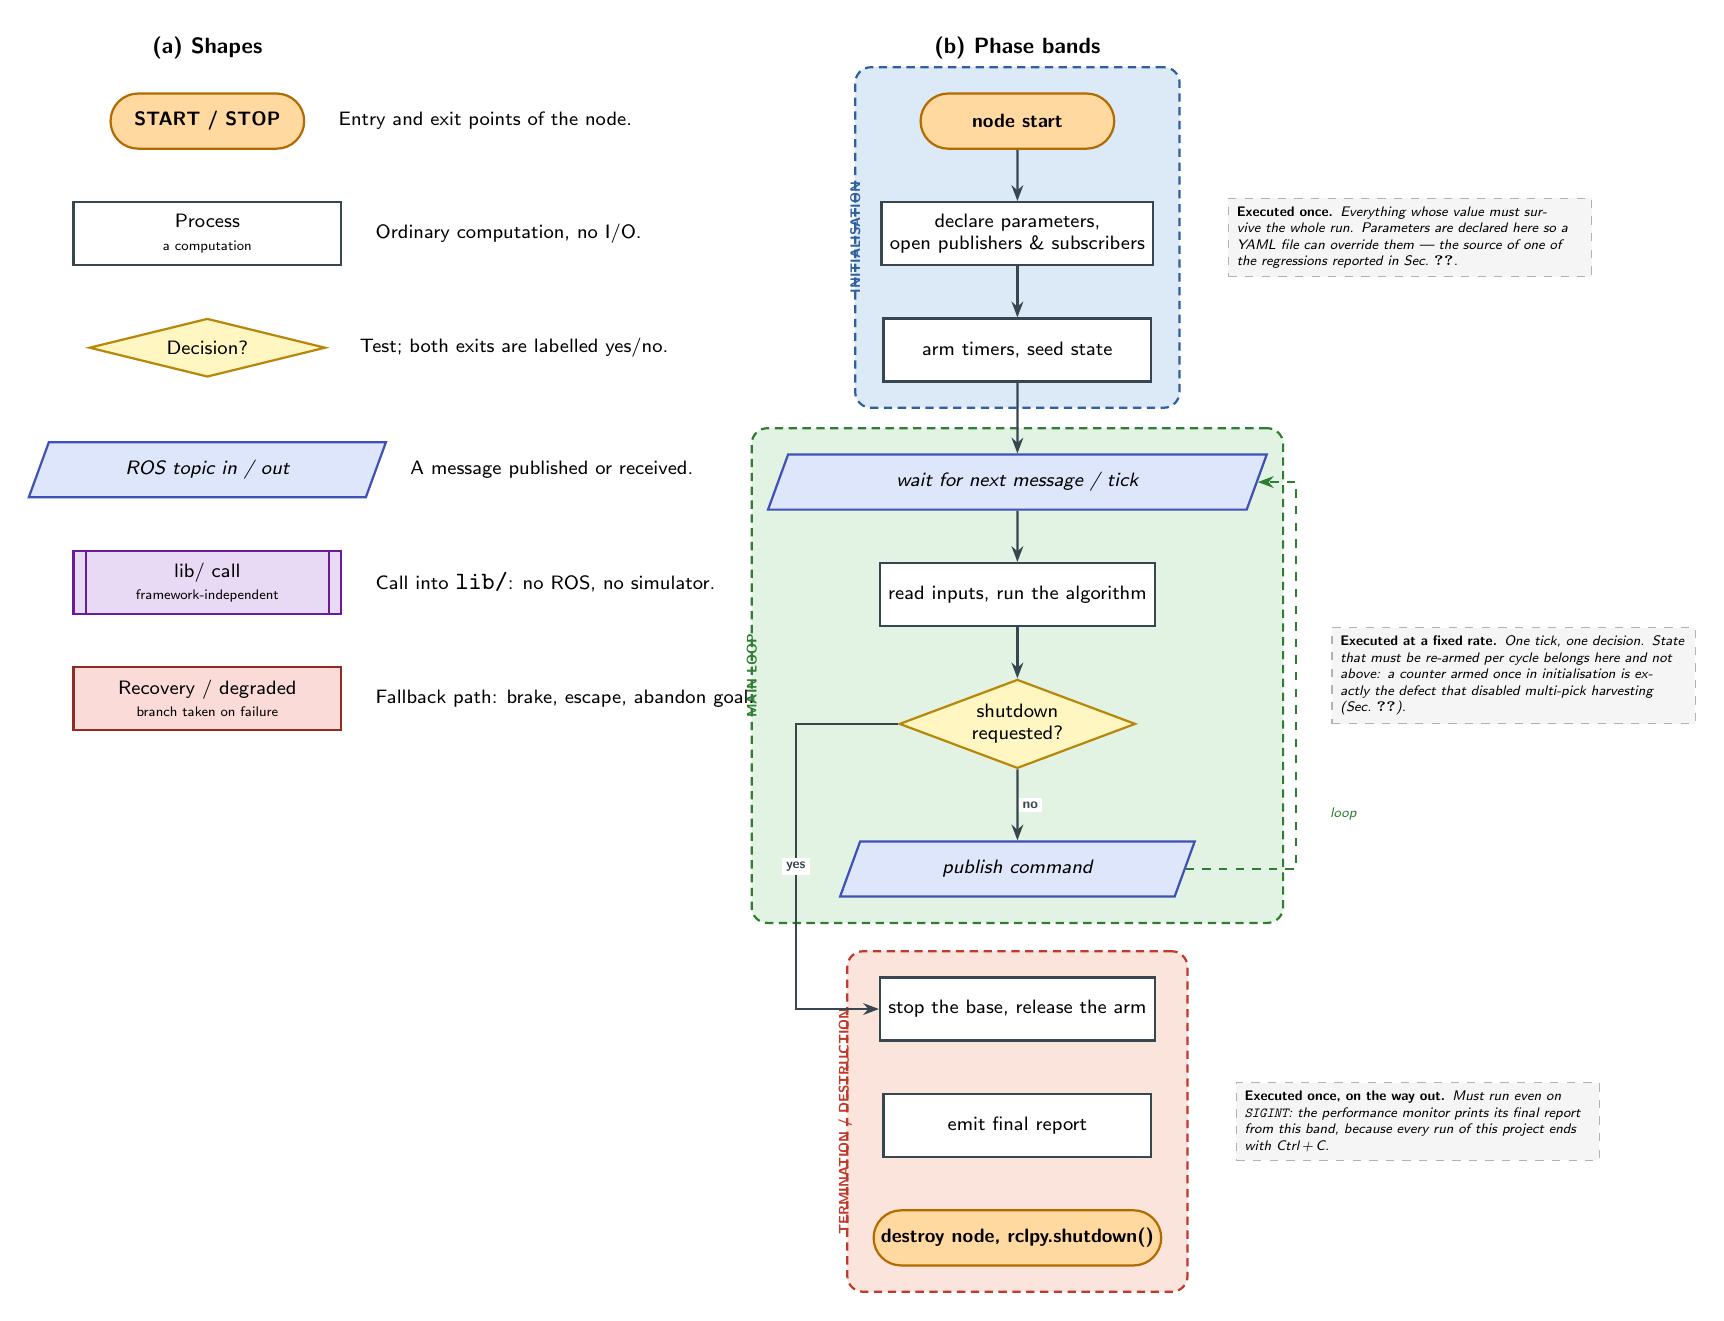
\begin{tikzpicture}[fcchain]

% ---------------------------------------------------------------------
%  LEFT BLOCK : the six node shapes
% ---------------------------------------------------------------------
\node[fcterm] (s1) {START / STOP};
\node[fcproc, below=of s1] (s2) {Process\\{\tiny a computation}};
\node[fcdec,  below=of s2] (s3) {Decision?};
\node[fcio,   below=8mm of s3] (s4) {ROS topic in / out};
\node[fcsub,  below=of s4] (s5) {lib/ call\\{\tiny framework-independent}};
\node[fcfail, below=of s5] (s6) {Recovery / degraded\\{\tiny branch taken on failure}};

\node[font=\sffamily\footnotesize\bfseries, above=3mm of s1] (shapeshdr)
     {(a) Shapes};

% shape annotations, to the right of each
\node[anchor=west, font=\sffamily\scriptsize, right=3mm of s1]
     {Entry and exit points of the node.};
\node[anchor=west, font=\sffamily\scriptsize, right=3mm of s2]
     {Ordinary computation, no I/O.};
\node[anchor=west, font=\sffamily\scriptsize, right=3mm of s3]
     {Test; both exits are labelled \textsf{yes}/\textsf{no}.};
\node[anchor=west, font=\sffamily\scriptsize, right=3mm of s4]
     {A message published or received.};
\node[anchor=west, font=\sffamily\scriptsize, right=3mm of s5]
     {Call into \filename{lib/}: no ROS, no simulator.};
\node[anchor=west, font=\sffamily\scriptsize, right=3mm of s6]
     {Fallback path: brake, escape, abandon goal.};

% ---------------------------------------------------------------------
%  RIGHT BLOCK : the three phase bands
% ---------------------------------------------------------------------
\node[fcterm, right=78mm of s1] (p0) {node start};
\node[fcproc, below=of p0] (p1) {declare parameters,\\open publishers \& subscribers};
\node[fcproc, below=of p1] (p2) {arm timers, seed state};

\node[fcio,   below=9mm of p2] (p3) {wait for next message / tick};
\node[fcproc, below=of p3] (p4) {read inputs, run the algorithm};
\node[fcdec,  below=of p4] (p5) {shutdown\\requested?};
\node[fcio,   below=9mm of p5] (p6) {publish command};

\node[fcproc, below=10mm of p6] (p7) {stop the base, release the arm};
\node[fcproc, below=of p7] (p8) {emit final report};
\node[fcterm, below=of p8] (p9) {destroy node, rclpy.shutdown()};

\draw[fcline] (p0) -- (p1);
\draw[fcline] (p1) -- (p2);
\draw[fcline] (p2) -- (p3);
\draw[fcline] (p3) -- (p4);
\draw[fcline] (p4) -- (p5);
\draw[fcline] (p5) -- node[fclab,right] {no} (p6);
\draw[fcback] (p6.east) -- ++(14mm,0) |- (p3.east);
\node[font=\sffamily\tiny\itshape, text=phaseMainLine]
     at ($(p6.east)+(20mm,7mm)$) {loop};
\draw[fcline] (p5.west) -- ++(-13mm,0) |- node[fclab,pos=0.25] {yes} (p7.west);

\node[font=\sffamily\footnotesize\bfseries, above=3mm of p0] {(b) Phase bands};

% ---- the bands themselves, on the background layer -------------------
\begin{scope}[on background layer]
  \phaseband{bandinit}{INITIALISATION}{phaseInitLine}{(p0)(p1)(p2)}{bi}
  \phaseband{bandmain}{MAIN LOOP}{phaseMainLine}{(p3)(p4)(p5)(p6)}{bm}
  \phaseband{bandend}{TERMINATION / DESTRUCTION}{phaseEndLine}{(p7)(p8)(p9)}{be}
\end{scope}

% ---- band annotations ------------------------------------------------
\node[fcnote, right=6mm of bi.east, anchor=west, text width=44mm]
     {\textbf{Executed once.} Everything whose value must survive the
      whole run. Parameters are declared here so a YAML file can
      override them --- the source of one of the regressions reported in
      Sec.~\ref{sec:regression}.};
\node[fcnote, right=6mm of bm.east, anchor=west, text width=44mm]
     {\textbf{Executed at a fixed rate.} One tick, one decision. State
      that must be re-armed per cycle belongs here and not above: a
      counter armed once in initialisation is exactly the defect that
      disabled multi-pick harvesting (Sec.~\ref{sec:phaseB_mission}).};
\node[fcnote, right=6mm of be.east, anchor=west, text width=44mm]
     {\textbf{Executed once, on the way out.} Must run even on
      \texttt{SIGINT}: the performance monitor prints its final report
      from this band, because every run of this project ends with
      Ctrl\,+\,C.};

\end{tikzpicture}
\caption{The flowchart language used throughout this report, defined
once. (a) The six node shapes: two are specific to a robotics stack ---
a \emph{ROS topic} shape, so the boundary with the middleware is
visible, and a \emph{library call} shape, so the boundary with the
framework-independent algorithm layer is visible. (b) The three phase
bands into which every later flowchart is partitioned. The banding is
functional rather than decorative: two of the defects analysed in this
report are cases of code placed in the wrong band.}
\label{fig:legend}
\end{figure*}


\subsection{Report structure}

Sec.~\ref{sec:related} reviews the literature each algorithm is drawn
from. Sec.~\ref{sec:environment} specifies the toolchain, the exact
software versions, and the installation procedure.
Sections~\ref{sec:phaseA}--\ref{sec:phaseA_results} present \phaseA{}
(Webots) in full, subsystem by subsystem.
Sections~\ref{sec:phaseB}--\ref{sec:regression} present \phaseB{}
(ROS~2 / Gazebo) in the same order, so the two phases can be read side
by side. Sec.~\ref{sec:swot} gives the SWOT analysis of every method.
Sec.~\ref{sec:results} reports the measured results,
Sec.~\ref{sec:discussion} discusses the limitations and what they imply
for a physical deployment, and Sec.~\ref{sec:conclusion} concludes.
Appendix~\ref{app:reproduce} gives the commands to reproduce every
experiment; Appendix~\ref{app:parameters} tabulates every tuned
parameter with its justification; Appendix~\ref{app:topics} gives the
full topic contract; Appendix~\ref{app:troubleshooting} collects the
failure modes encountered and their diagnosis.

%% =====================================================================
%%  Related Work
%%  SCOPE: Literature each algorithm is drawn from, and what this work adds.
%% =====================================================================
\section{Related Work}
\label{sec:related}

\emph{[Section in preparation.]}

% =====================================================================
%  Development Environment and Toolchain
%  SCOPE: Exact versions, installation, build and launch procedures.
% =====================================================================
\section{Development Environment and Toolchain}
\label{sec:environment}

This section specifies the software environment precisely enough that
every result in this report can be regenerated on a clean machine. It is
placed before the technical chapters deliberately: several of the
defects analysed later are consequences of version-specific behaviour
(a deprecated Gazebo service, a build mode that resolves entry points
through a symbolic link), and those are not intelligible without knowing
exactly what was running.

\subsection{Hardware and operating system}

All development and all reported experiments were carried out on a
single workstation, Table~\ref{tab:hardware}. No GPU-accelerated
inference is used anywhere in the stack; the only GPU consumer is the
simulator's rendering pipeline, which also serves the simulated lidar
(Sec.~\ref{sec:phaseB_twin} explains why that matters).

\begin{table}[!t]
\caption{Development and experiment platform}
\label{tab:hardware}
\centering\footnotesize
\begin{tabular}{@{}ll@{}}
\toprule
\textbf{Item} & \textbf{Value}\\
\midrule
Machine            & HP EliteBook laptop\\
Operating system   & Ubuntu 24.04 LTS (Noble Numbat)\\
Display server     & Wayland, with Qt forced to XCB\\
Python             & 3.12 (system interpreter)\\
Project storage    & external volume, mounted under \filename{/mnt}\\
\bottomrule
\end{tabular}
\end{table}

The display server is worth recording. Gazebo's GUI detects Wayland and
falls back to the XCB Qt platform plugin, printing
\texttt{Detected Wayland. Setting Qt to use the xcb plugin} at every
start. This is benign in itself, but it is one reason the GUI
camera-tracking behaviour differs from the documented default, which
motivated the camera watchdog described in Sec.~\ref{sec:phaseB_twin}.

\subsection{Software versions}

Table~\ref{tab:versions} lists every component whose version affects the
results. Two entries are load-bearing:

\begin{itemize}[leftmargin=*,itemsep=1pt,topsep=2pt]
  \item \textbf{Gazebo Harmonic (gz-sim 8.11.0)} deprecated the
        \topicname{gui/follow} service in favour of the
        \topicname{gui/track} topic. Code written against the older API
        fails silently --- the camera simply never locks onto the robot
        --- which cost one full debugging cycle
        (Appendix~\ref{app:troubleshooting}).
  \item \textbf{\texttt{colcon build -{}-symlink-install}} resolves
        console-script entry points through an egg-link back into
        \filename{src/}. When that metadata goes missing, every node
        dies at import with \texttt{PackageNotFoundError} --- fifteen
        identical tracebacks that name the symptom and not the cause.
        The launch wrapper tests for this explicitly before starting
        anything.
\end{itemize}

\begin{table}[!t]
\caption{Software components and versions}
\label{tab:versions}
\centering\footnotesize
\begin{tabular}{@{}lll@{}}
\toprule
\textbf{Component} & \textbf{Version} & \textbf{Role}\\
\midrule
Webots                        & R2025a          & \phaseA{} simulator\\
ROS~2                         & Jazzy Jalisco   & \phaseB{} middleware\\
Gazebo Sim                    & Harmonic 8.11.0 & \phaseB{} simulator\\
\texttt{ros\_gz\_sim}         & Jazzy           & spawn, world launch\\
\texttt{ros\_gz\_bridge}      & Jazzy           & topic bridging\\
\texttt{webots\_ros2\_driver} & Jazzy           & \phaseA{}$\rightarrow$ROS\\
RViz~2                        & Jazzy           & visualisation\\
NumPy                         & system package  & grids, scan matching\\
colcon                        & system package  & build tool\\
Physics engine                & DART (default)  & 1\,ms step\\
\bottomrule
\end{tabular}
\end{table}

\subsection{Installation}

Listing~\ref{lst:install} gives the complete installation from a clean
Ubuntu 24.04. The ROS~2 and Gazebo repositories are added first; the
\texttt{ros-jazzy-ros-gz} metapackage pulls in both the bridge and the
simulator integration.

\begin{lstlisting}[style=bash,caption={Full installation on a clean
Ubuntu 24.04.},label={lst:install}]
# --- 1. ROS 2 Jazzy -------------------------------------
sudo apt update && sudo apt install -y \
     software-properties-common curl
sudo add-apt-repository universe
sudo curl -sSL -o /usr/share/keyrings/ros-archive-keyring.gpg \
  https://raw.githubusercontent.com/ros/rosdistro/master/ros.key
echo "deb [signed-by=/usr/share/keyrings/\
ros-archive-keyring.gpg] \
http://packages.ros.org/ros2/ubuntu noble main" \
     | sudo tee /etc/apt/sources.list.d/ros2.list
sudo apt update
sudo apt install -y ros-jazzy-desktop

# --- 2. Gazebo Harmonic + the ROS 2 bridge --------------
sudo apt install -y ros-jazzy-ros-gz \
                    ros-jazzy-ros-gz-sim \
                    ros-jazzy-ros-gz-bridge

# --- 3. Webots R2025a (Phase A) -------------------------
sudo apt install -y ros-jazzy-webots-ros2
# plus the Webots R2025a .deb from cyberbotics.com

# --- 4. Build tooling and Python dependencies -----------
sudo apt install -y python3-colcon-common-extensions \
                    python3-numpy python3-opencv

# --- 5. The report toolchain (optional) -----------------
sudo apt install -y texlive-latex-extra texlive-publishers \
                    texlive-science
\end{lstlisting}

\subsection{Workspace layout and build}

The ROS~2 workspace contains five packages, Table~\ref{tab:packages}.
The split is not cosmetic: \texttt{youbot\_control} holds the algorithms
and the control nodes and depends on \emph{no} simulator, while
\texttt{youbot\_gazebo} and \texttt{youbot\_webots} are thin,
simulator-specific shells. This is what allowed \phaseA{} to be reused
in \phaseB{} rather than rewritten (Sec.~\ref{sec:architecture}).

\begin{table}[!t]
\caption{ROS~2 workspace packages and their dependencies}
\label{tab:packages}
\centering\footnotesize
\begin{tabular}{@{}p{0.24\columnwidth}p{0.66\columnwidth}@{}}
\toprule
\textbf{Package} & \textbf{Depends on}\\
\midrule
\texttt{youbot\_control} &
  \texttt{rclpy}, \texttt{geometry\_msgs}, \texttt{sensor\_msgs},
  \texttt{nav\_msgs}, \texttt{tf2\_ros},
  \texttt{visualization\_msgs}, \texttt{numpy}\\
\texttt{youbot\_slam} &
  \texttt{rclpy}, \texttt{nav\_msgs}, \texttt{sensor\_msgs},
  \texttt{geometry\_msgs}, \texttt{tf2\_ros},
  \texttt{youbot\_control}\\
\texttt{youbot\_gazebo} &
  \texttt{youbot\_control}, \texttt{youbot\_bringup},
  \texttt{ros\_gz\_sim}, \texttt{ros\_gz\_bridge},
  \texttt{robot\_state\_publisher}, \texttt{rviz2}\\
\texttt{youbot\_bringup} &
  \texttt{youbot\_control}, \texttt{launch}, \texttt{launch\_ros},
  \texttt{rviz2}, \texttt{robot\_state\_publisher}\\
\texttt{youbot\_webots} &
  \texttt{webots\_ros2\_driver}, \texttt{youbot\_control},
  \texttt{rclpy}\\
\bottomrule
\end{tabular}
\end{table}

Note the direction of the arrows: no package containing an algorithm
depends on a simulator, and no simulator package is depended upon by
another. \texttt{youbot\_slam} depends on \texttt{youbot\_control} only
to reuse the occupancy-grid and scan-matching libraries.

\begin{lstlisting}[style=bash,caption={Cloning and building.},
label={lst:build}]
git clone https://github.com/\
franckarmandjosiasEinstein-bit/ROS2_stage.git
cd ROS2_stage
source /opt/ros/jazzy/setup.bash
colcon build --symlink-install
source install/setup.bash
\end{lstlisting}

\texttt{-{}-symlink-install} is used so that editing a Python node takes
effect without a rebuild, which matters when one simulation run costs
half an hour of wall time. Its price is the entry-point fragility
described above; if that appears, a plain \texttt{colcon build} writes
real distribution metadata and removes the dependency on
\filename{src/} entirely.

\subsection{Running a simulation}

Every experiment is launched through one wrapper script,
\filename{src/youbot\_gazebo/scripts/run.sh}, rather than through
\texttt{ros2 launch} directly. The wrapper exists because of three
concrete failures, each of which cost at least one run:

\begin{enumerate}[leftmargin=*,itemsep=1pt,topsep=2pt]
  \item \textbf{Gazebo does not die on Ctrl\,+\,C.} A surviving
        \texttt{gz sim} keeps publishing an old \topicname{clock}; the
        next run then has two clocks, RViz thrashes, and the GUI can
        attach to a ghost world with no robot in it. The wrapper
        installs a cleanup trap and afterwards \emph{verifies} that
        nothing survived, printing the command line of any process it
        could not match rather than leaving it to be inferred from the
        next run misbehaving.
  \item \textbf{Gazebo rewrites its GUI configuration on every exit}
        with wherever the camera was left, and reads it back in
        preference to the world's \texttt{<gui>} pose. A run started
        after the camera was parked on empty space opens blind. The
        wrapper deletes \filename{\textasciitilde/.gz/sim/8/gui.config}
        before starting.
  \item \textbf{Silent build breakage}, via the entry-point check
        described above.
\end{enumerate}

The wrapper then runs the pre-flight regression suite
(Sec.~\ref{sec:regression}) and refuses to start if any check fails:
about one second of pure Python weighed against thirty minutes of
simulation.

\begin{lstlisting}[style=bash,caption={The supported launch
configurations.},label={lst:run}]
# Level 2 -- ground-truth pose, no SLAM (baseline)
./src/youbot_gazebo/scripts/run.sh

# Level 3 -- homemade SLAM in the loop
./src/youbot_gazebo/scripts/run.sh slam

# Level 3 -- calibrated dead reckoning, SLAM disabled
#            (the production configuration, Sec. V-E)
./src/youbot_gazebo/scripts/run.sh slam \
      slam:=false pose_topic:=odom_calibrated

# Headless, for batch runs
./src/youbot_gazebo/scripts/run.sh slam gui:=false
\end{lstlisting}

A correct start prints three markers, in this order. Their absence is
the fastest way to detect that a stale build is being run --- a mistake
made twice during this project, both times producing a log that looked
plausible and was measuring the wrong binary:

\begin{lstlisting}[style=bash]
[run.sh] pre-flight: all 191 checks passed.
[mapping_node] mapping_node up: /scan + /odom -> /map
               (inflated, for planning) + /map_raw (evidence)
[perf_monitor] perf_monitor up: timing, throughput and
               where the time goes.
\end{lstlisting}

\subsection{Running \phaseA{} (Webots)}

\phaseA{} is self-contained and does not require ROS. Webots is opened
on one of the two worlds and the \texttt{controller} field of the YouBot
node selects which of the fifteen controllers runs
(Sec.~\ref{sec:phaseA}). The \texttt{youbot\_webots} package exists only
to expose the same robot to ROS~2 through
\texttt{webots\_ros2\_driver}; it was used to confirm that the algorithm
layer behaved identically under both simulators before the Gazebo twin
was built.

\begin{lstlisting}[style=bash,caption={Launching \phaseA{}.},
label={lst:webots}]
# Standalone Webots (no ROS): open the world, then choose
# the controller in the scene tree.
webots worlds/smart_agriculture.wbt
webots worlds/greenhouse.wbt

# The same robot exposed to ROS 2 (bridge validation)
ros2 launch youbot_webots webots.launch.py
\end{lstlisting}

\subsection{Version control and reproducibility}

The two phases live in two repositories: the Webots prototype in
\texttt{Projet}, and the ROS~2 stack in \texttt{ROS2\_stage}. Every
result quoted in Sec.~\ref{sec:results} names the commit it was produced
from, because two of the analyses in this report compare runs that
differ by a single parameter file. Appendix~\ref{app:reproduce} lists
those commits alongside the exact command and the expected output.


% ---- PHASES A & B : the autonomous platform ---------------------------
%  Kept in full. These are completed, measured subsystems, and the
%  report's own argument in Sec. \ref{sec:extension} depends on their
%  results being on the record rather than asserted.
%% =====================================================================
%%  Phase A --- Webots Prototype: Overview
%%  SCOPE: Why Webots first; the fifteen controllers and their dependency order.
%% =====================================================================
\section{Phase A --- Webots Prototype: Overview}
\label{sec:phaseA}

\emph{[Section in preparation.]}

%% =====================================================================
%%  World Modelling and the Procedural Greenhouse
%%  SCOPE: smart\_agriculture.wbt, greenhouse.wbt, world\_manager supervisor.
%% =====================================================================
\subsection{World Modelling and the Procedural Greenhouse}
\label{sec:phaseA_world}

\emph{[Section in preparation.]}

%% =====================================================================
%%  Locomotion: Mecanum Kinematics and Odometry
%%  SCOPE: base\_test, wheel\_test, odom\_test; the four-wheel mapping.
%% =====================================================================
\subsection{Locomotion: Mecanum Kinematics and Odometry}
\label{sec:phaseA_locomotion}

\emph{[Section in preparation.]}

%% =====================================================================
%%  Perception: Lidar and Colour Vision
%%  SCOPE: lidar\_test, vision\_test; blob detection and ground projection.
%% =====================================================================
\subsection{Perception: Lidar and Colour Vision}
\label{sec:phaseA_perception}

\emph{[Section in preparation.]}

% =====================================================================
%  Mapping and Localisation
%  SCOPE: mapping.py (log-odds grid, Bresenham, inflation),
%         localization.py (odometry, likelihood-field scan matching),
%         exploration.py (frontier extraction).
% =====================================================================
\subsection{Mapping and Localisation}
\label{sec:phaseA_mapping}

\subsubsection{The representation: a log-odds occupancy grid}

The map is a $100 \times 100$ grid covering the \SI{10}{m} arena at
\SI{0.10}{m} resolution, following Moravec and Elfes
\cite{moravec1985occupancy}. Each cell carries not a binary state but a
\emph{log-odds} value $\ell$, the logarithm of the ratio between the
probability that the cell is occupied and the probability that it is
free:

\begin{equation}
\ell(c) = \log \frac{P(c\ \text{occupied})}{P(c\ \text{free})}.
\label{eq:logodds}
\end{equation}

The reason for the logarithm is arithmetic, not aesthetic. In
probability space, fusing independent observations requires a product
and a renormalisation; in log-odds space it is an addition
\cite{thrun2005probabilistic}. Fusing a scan therefore becomes a sweep
of \texttt{+=} over an array, which is both fast and numerically
untroubled. Two constants define the sensor model actually used:

\begin{center}\footnotesize
\begin{tabular}{@{}llr@{}}
\toprule
\param{L\_OCC}  & added where a beam terminates & $+0.85$\\
\param{L\_FREE} & added to every cell the beam crosses & $-0.40$\\
\param{L\_CLAMP} & saturation bound on $|\ell|$ & $5.0$\\
\param{L\_OCC\_THRESHOLD} & $\ell$ above which a cell is ``occupied'' & $0.5$\\
\bottomrule
\end{tabular}
\end{center}

Three deliberate asymmetries are encoded in those four numbers.

\textbf{Occupied evidence is worth more than free evidence}
($0.85$ against $0.40$). A beam that stops has made a positive
measurement of a surface; a beam that passes through has only failed to
find one. Making them equal produces a map that erodes thin obstacles,
because a gutter edge is crossed by many more passing beams than
terminating ones.

\textbf{The belief is clamped.} Without \param{L\_CLAMP}, a wall seen
five hundred times reaches $\ell = 400$ and needs a thousand
contradicting observations to be forgotten. The map would then be unable
to react to a moving worker who parks somewhere and later leaves. The
clamp at $\pm 5$ keeps roughly ten contradicting scans sufficient to
flip a cell, which is the right time constant for obstacles moving at
\SI{0.3}{m/s} in a \SI{10}{m} arena.

\textbf{The occupancy threshold is not zero but $+0.5$.} A cell must
accumulate net positive evidence, not merely non-negative evidence,
before the planner is told to avoid it. This is the cheapest available
defence against single-beam noise.

\subsubsection{Integrating one scan: exact ray casting}

For each of the 360 beams the mapper computes the world-frame bearing
$\alpha = \psi + \big(\tfrac{\mathrm{fov}}{2} - i\,\Delta\big)$, decides
whether the beam terminated on a surface ($\texttt{dist}$ finite and
below \param{max\_range}), and walks the integer line from the robot
cell to the endpoint cell with Bresenham's algorithm
\cite{bresenham1965algorithm}:

\begin{lstlisting}[style=python]
for (cc, cr) in self._bresenham(r0c, r0r, ec, er):
    if cc == ec and cr == er:
        break            # stop BEFORE the endpoint
    self.log_odds[cr, cc] += L_FREE
if hit:
    self.log_odds[er, ec] += L_OCC
\end{lstlisting}

The \texttt{break} is not decoration. Without it the endpoint cell
receives \param{L\_FREE} on the same pass that gives it
\param{L\_OCC}, and the wall's net evidence per scan falls from $+0.85$
to $+0.45$ --- halving the convergence rate for no reason at all. It is
a one-line detail that is invisible in the code review and obvious in
the resulting map.

\paragraph{A rejected optimisation, and why it was rejected}
The per-beam Python loop is the slowest part of \phaseA{}. A numpy
rewrite was implemented and benchmarked: sample each ray at half-cell
intervals and scatter with \texttt{np.add.at}. It was measured to be
\emph{both slower and less accurate} --- slower because
\texttt{np.add.at} is not vectorised internally over duplicate indices,
and less accurate because half-cell sampling can skip the very cell a
beam grazes, eroding occupied cells along oblique walls. The exact
sweep was kept, and the mapper was instead run once every
\param{INTEGRATE\_EVERY} $= 4$ control ticks, which costs nothing in map
quality because the robot moves less than \SI{4}{cm} in that interval.
Recording a rejected optimisation is as much part of the engineering
record as recording an accepted one.

\paragraph{A near-range gate}
Beams shorter than \param{min\_range} $= \SI{0.25}{m}$ are discarded
entirely. At that distance the return is either the robot's own
structure or noise, and integrating it stamps a permanent obstacle onto
the cell the robot is standing in --- after which the planner cannot
find a path out of it.

\subsubsection{From belief to plan: thresholding and inflation}

The planner cannot consume log-odds. \texttt{update\_grid\_from\_log\_odds}
produces the binary planning grid in two steps: threshold at
\param{L\_OCC\_THRESHOLD}, then dilate every occupied cell by a disc of
radius \param{inflation}.

Inflation is what turns a map of the \emph{world} into a map of the
\emph{robot's configuration space} \cite{lozanoperez1983spatial}. Once
obstacles are grown by the robot's own radius, the planner may treat the
robot as a dimensionless point, and any path it returns through free
cells is collision-free for the real body. In \phaseA{} the radius is
\SI{0.32}{m}, chosen to cover the YouBot half-diagonal of
$\sqrt{0.29^2 + 0.19^2} = \SI{0.347}{m}$ with a small deliberate
shortfall so that the \SI{1.2}{m} aisles remain traversable.

That choice --- a disc sized on the half-diagonal --- is exactly the
approximation that \phaseB{} later had to abandon. A disc of
\SI{0.347}{m} is correct for a robot that may be rotated arbitrarily,
but it is \SI{16}{cm} too conservative sideways, and in the
\SI{0.80}{m} aisles of the Phase~B greenhouse that conservatism is the
difference between a passable lane and an impassable one. The rectangle
model of Sec.~\ref{sec:safety} replaces it.

The dilation itself is done by shifted whole-array \texttt{OR}s rather
than a per-cell neighbourhood scan:

\begin{lstlisting}[style=python]
for dr in range(-radius, radius + 1):
    for dc in range(-radius, radius + 1):
        if dr*dr + dc*dc > radius*radius:
            continue
        out[r_dst0:r_dst1, c_dst0:c_dst1] |= \
            occupied[r_src0:r_src1, c_src0:c_src1]
\end{lstlisting}

which is $O(\text{radius}^2)$ array operations instead of
$O(\text{cells} \times \text{radius}^2)$ scalar ones --- for a
$100\times100$ grid and a 3-cell radius, 45 array \texttt{OR}s in place
of 450\,000 Python iterations.

% =====================================================================
%  Log-odds occupancy mapping from one lidar scan -- Phase A (mapping.py)
%  Two-column float: the beam loop and the grid pipeline sit side by side.
% =====================================================================
\begin{figure*}[!t]
\centering
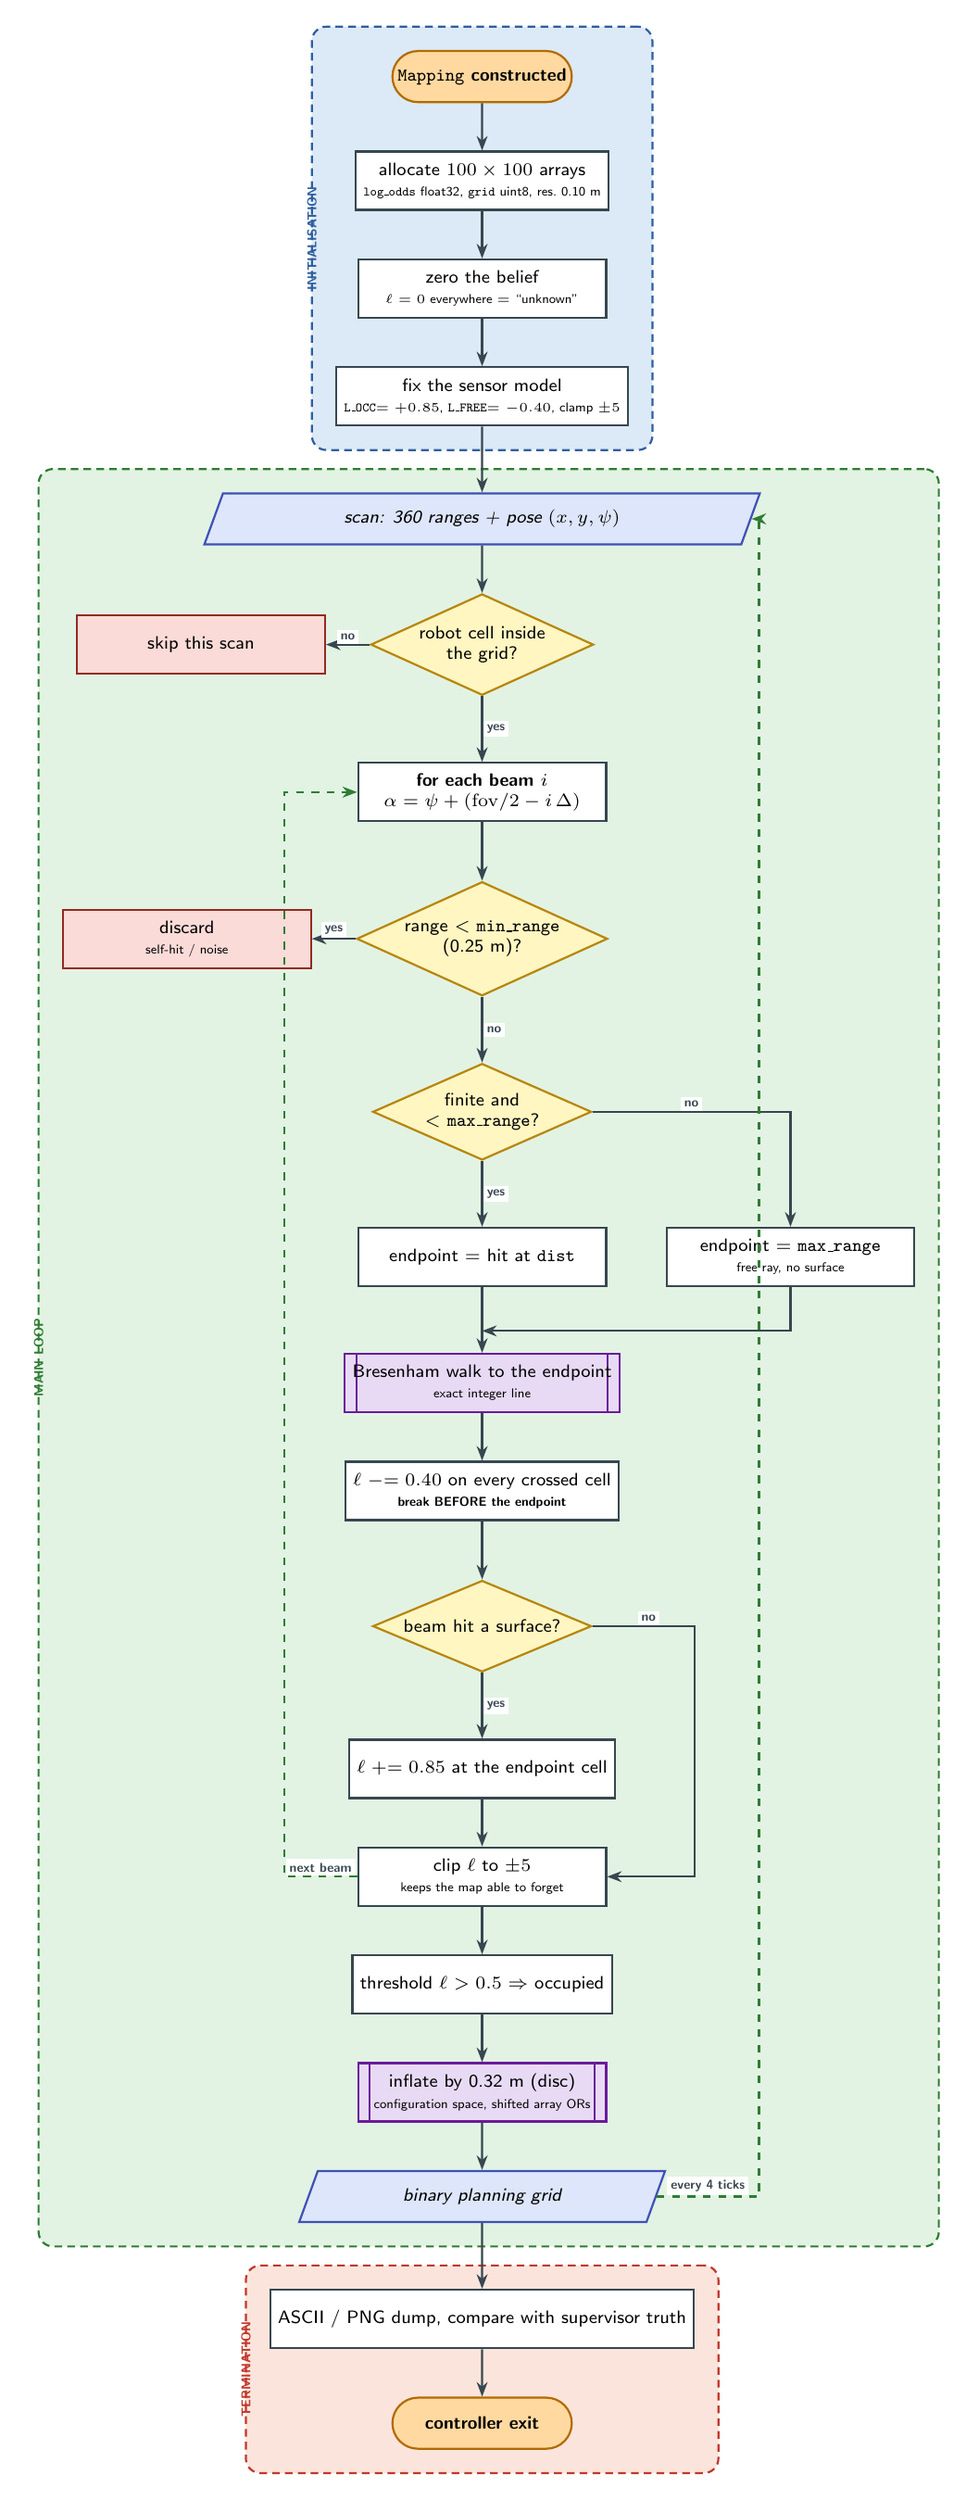
\begin{tikzpicture}[fcchain]

% ---------------- INITIALISATION (left column) ------------------------
\node[fcterm] (m0) {\texttt{Mapping} constructed};
\node[fcproc, below=of m0] (m1)
     {allocate $100\times100$ arrays\\
      {\tiny \texttt{log\_odds} float32, \texttt{grid} uint8, res.\ 0.10 m}};
\node[fcproc, below=of m1] (m2)
     {zero the belief\\{\tiny $\ell = 0$ everywhere $=$ ``unknown''}};
\node[fcproc, below=of m2] (m3)
     {fix the sensor model\\
      {\tiny \texttt{L\_OCC}$=+0.85$, \texttt{L\_FREE}$=-0.40$, clamp $\pm5$}};

% ---------------- MAIN LOOP (left column) -----------------------------
\node[fcio, below=9mm of m3] (n0) {scan: 360 ranges + pose $(x,y,\psi)$};
\node[fcdec, below=of n0] (n1) {robot cell inside\\the grid?};
\node[fcfail, left=6mm of n1] (n1b) {skip this scan};
\node[fcproc, below=9mm of n1] (n2)
     {\textbf{for each beam $i$}\\
      $\alpha = \psi + (\mathrm{fov}/2 - i\,\Delta)$};
\node[fcdec, below=8mm of n2] (n3)
     {range $<$ \texttt{min\_range}\\(0.25 m)?};
\node[fcfail, left=6mm of n3] (n3b) {discard\\{\tiny self-hit / noise}};
\node[fcdec, below=9mm of n3] (n4) {finite and\\$<$ \texttt{max\_range}?};
\node[fcproc, below=9mm of n4] (n5)
     {endpoint $= $ hit at \texttt{dist}};
\node[fcproc, right=8mm of n5] (n5b)
     {endpoint $= $ \texttt{max\_range}\\{\tiny free ray, no surface}};

% ---------------- MAIN LOOP (right column) ----------------------------
\node[fcsub, below=9mm of n5] (n6)
     {Bresenham walk to the endpoint\\{\tiny exact integer line}};
\node[fcproc, below=of n6] (n7)
     {$\ell \mathrel{-}= 0.40$ on every crossed cell\\
      {\tiny \textbf{break BEFORE the endpoint}}};
\node[fcdec, below=8mm of n7] (n8) {beam hit a surface?};
\node[fcproc, below=9mm of n8] (n9) {$\ell \mathrel{+}= 0.85$ at the endpoint cell};
\node[fcproc, below=of n9] (n10)
     {clip $\ell$ to $\pm 5$\\{\tiny keeps the map able to forget}};
\node[fcproc, below=of n10] (n11)
     {threshold $\ell > 0.5 \Rightarrow$ occupied};
\node[fcsub, below=of n11] (n12)
     {inflate by 0.32 m (disc)\\{\tiny configuration space, shifted array ORs}};
\node[fcio, below=of n12] (n13) {binary planning grid};

% ---------------- TERMINATION -----------------------------------------
\node[fcproc, below=9mm of n13] (p0)
     {ASCII / PNG dump, compare with supervisor truth};
\node[fcterm, below=of p0] (p1) {controller exit};

% ---------------- edges ------------------------------------------------
\draw[fcline] (m0) -- (m1);
\draw[fcline] (m1) -- (m2);
\draw[fcline] (m2) -- (m3);
\draw[fcline] (m3) -- (n0);
\draw[fcline] (n0) -- (n1);
\draw[fcline] (n1) -- node[fclab,above] {no} (n1b);
\draw[fcline] (n1) -- node[fclab,right] {yes} (n2);
\draw[fcline] (n2) -- (n3);
\draw[fcline] (n3) -- node[fclab,above] {yes} (n3b);
\draw[fcline] (n3) -- node[fclab,right] {no} (n4);
\draw[fcline] (n4) -- node[fclab,right] {yes} (n5);
\draw[fcline] (n4.east) -| node[fclab,pos=0.25,above] {no} (n5b.north);
\draw[fcline] (n5) -- (n6);
\draw[fcline] (n5b.south) |- ($(n6.north)+(0,3mm)$);
\draw[fcline] (n6) -- (n7);
\draw[fcline] (n7) -- (n8);
\draw[fcline] (n8) -- node[fclab,right] {yes} (n9);
\draw[fcline] (n8.east) -- ++(14mm,0)
      node[fclab,pos=0.55,above] {no} |- (n10.east);
\draw[fcline] (n9) -- (n10);
\draw[fcback] (n10.west) -- ++(-10mm,0)
      node[fclab,pos=0.5,above] {next beam} |- (n2.west);
\draw[fcline] (n10) -- (n11);
\draw[fcline] (n11) -- (n12);
\draw[fcline] (n12) -- (n13);
\draw[fcback] (n13.east) -- ++(14mm,0)
      node[fclab,pos=0.5,above] {every 4 ticks} |- (n0.east);
\draw[fcline] (n13) -- (p0);
\draw[fcline] (p0) -- (p1);

% ---------------- phase bands ------------------------------------------
\begin{scope}[on background layer]
  \phaseband{bandinit}{INITIALISATION}{phaseInitLine}{(m0)(m1)(m2)(m3)}{ma}
  \phaseband{bandmain}{MAIN LOOP}{phaseMainLine}
    {(n0)(n1)(n1b)(n2)(n3)(n3b)(n4)(n5)(n5b)(n6)(n7)(n8)(n9)(n10)(n11)(n12)(n13)}{mb}
  \phaseband{bandend}{TERMINATION}{phaseEndLine}{(p0)(p1)}{mc}
\end{scope}

\end{tikzpicture}
\caption{Log-odds occupancy mapping from a single lidar scan
(\phaseA{}, \filename{mapping.py}). The initialisation band allocates
the belief array and fixes the sensor model; nothing in the loop depends
on scene content, so the same code maps the \phaseA{} arena and, ported
unchanged in substance, the \phaseB{} greenhouse. Two details in the
main loop carry disproportionate weight: the Bresenham walk stops
\emph{before} the endpoint, so a wall gains the full $+0.85$ per scan
instead of a net $+0.45$; and the clamp at $\pm5$ is what allows a cell
vacated by a moving worker to be forgotten within about ten scans. The
inflation step at the bottom is the boundary between a map of the world
and a map of the robot's configuration space.}
\label{fig:flow_mapping}
\end{figure*}


\subsubsection{Localisation, part 1: dead reckoning}

\filename{localization.py} first provides a GPS-free pose by integrating
the mecanum forward kinematics of Sec.~\ref{sec:phaseA_locomotion} over
the four wheel encoders. It is exact in the absence of slip and its
error is unbounded and monotone in its presence. Every metre driven adds
error that is never removed, which is the entire justification for what
follows.

\subsubsection{Localisation, part 2: likelihood-field scan matching}

The corrector is a \emph{correlative scan matcher}
\cite{olson2009correlative}: given a pose prior from odometry, search a
small window of $(\Delta x, \Delta y, \Delta\psi)$ offsets for the one
that best explains the current scan against a reference map. The score
of a candidate pose is a likelihood field \cite{thrun2005probabilistic}:
project the scan endpoints into the map, look up each endpoint's
distance $d$ to the nearest obstacle surface, and sum a Gaussian,

\begin{equation}
S(x,y,\psi) = \sum_{k \in \text{beams}}
              \exp\!\left(-\frac{d_k^2}{2\sigma^2}\right),
\qquad \sigma = \SI{0.15}{m}.
\label{eq:likelihood}
\end{equation}

Three implementation decisions carry the performance, and each of them
was made after the naive version failed.

\paragraph{The distance field is seeded from surfaces, not from solids}
The first version computed distance-to-nearest-\emph{occupied-cell}.
This saturates: a scan shifted bodily \emph{inside} a large planting
basin still lands every endpoint on an occupied cell, scores a perfect
$d = 0$ everywhere, and the search has no gradient to climb. Real lidar
only ever sees obstacle \emph{boundaries}, so the breadth-first distance
transform is seeded from occupied cells that touch free space:

\begin{lstlisting}[style=python]
occ = grid > 0
free_neighbor[:-1, :] |= ~occ[1:, :]   # and the three other shifts
return occ & free_neighbor
\end{lstlisting}

Endpoints that drift into an obstacle interior are then penalised, and
the score surface acquires a genuine peak at the true pose.

\paragraph{Coarse-then-fine, with a cached beam layout}
The search runs a coarse pass ($\pm\SI{0.30}{m}$ in steps of
\SI{0.10}{m}, $\pm\SI{0.10}{rad}$ in steps of \SI{0.05}{rad}) followed
by a fine pass around the winner ($\pm\SI{0.06}{m}$ / \SI{0.02}{m},
$\pm\SI{0.04}{rad}$ / \SI{0.02}{rad}). That is $7^3 = 343$ candidates
plus $7^3$ again, rather than the $31^3 = 29\,791$ a single fine sweep
would need. Every beam is subsampled by \param{beam\_stride} $= 6$
(60 of 360 beams), and the subsampled indices and their local bearings
depend only on the scan geometry --- constant across all 686 candidates
--- so they are computed once and cached. The score itself is fully
vectorised, which measured about ten times faster than the equivalent
per-beam loop.

\paragraph{A strictly-better trust gate}
The corrected pose is accepted \emph{only if it scores strictly higher
than the prior}:

\begin{lstlisting}[style=python]
if score <= prior_score:
    return prior, prior_score
\end{lstlisting}

The reason is a failure that was observed rather than predicted. In a
region of long straight walls the score surface has a broad plateau: a
scan shifted along the wall explains the map exactly as well as the true
pose. Without the gate the search settles on an arbitrary point of that
plateau, the result is fed back into the odometry as a reset, and the
next iteration starts from a slightly worse prior --- a slow runaway
driven entirely by ties. Comparing with $\le$ rather than $<$ also
covers the degenerate case of an uninformative scan, where every
candidate scores identically and the search would otherwise adopt a
window-corner offset on no evidence at all.

This single line is, in retrospect, the most important defensive
decision in the localisation stack, and its \phaseB{} descendant is the
rule that a scan-matching estimate may never be trusted merely because
it exists (Sec.~\ref{sec:slam}, where the homemade matcher is shown to
be \emph{worse} than the prior it was meant to improve).

\subsubsection{Assembling the estimator}

\texttt{LocalizationEstimator} bundles the two behind one \texttt{pose()}
callable: odometry integrates every tick, and every
\param{correct\_every} $= 8$ ticks the scan matcher snaps the estimate
back onto the reference map and resets the odometry to the corrected
value. Between corrections the pose tracks the wheels; the drift is
bounded by the correction period rather than by the distance driven.
Because the interface is a single callable, the mission layer can be
switched between ground-truth GPS and this estimator by changing one
argument --- which is how the two were compared quantitatively.

\subsubsection{Frontier extraction: deciding where to look next}

\filename{exploration.py} closes the loop between the map and the
mission. Rather than patrolling a fixed waypoint list, the robot drives
to the boundary between known-free and unknown space
\cite{yamauchi1997frontier}. Working directly on the log-odds array,

\begin{align}
\text{free}(c)    &\iff \ell(c) < -0.5, \\
\text{unknown}(c) &\iff |\ell(c)| < 0.1, \\
\text{frontier}(c)&\iff \text{free}(c) \wedge
   \exists\, c' \in \mathcal{N}_4(c) : \text{unknown}(c').
\end{align}

The three-way test is why the log-odds array is kept rather than
discarded after thresholding: a binary grid cannot distinguish
``observed and empty'' from ``never observed'', and frontier exploration
is exactly the algorithm that needs that distinction.

Frontier cells are clustered by 4-connectivity, clusters smaller than
\param{min\_cluster} $= 4$ cells are dropped as noise, and each surviving
cluster contributes one goal. Two refinements matter:

\begin{itemize}[leftmargin=*,itemsep=1pt,topsep=2pt]
  \item The goal is the frontier cell \emph{nearest the robot}, never
        the cluster centroid. For a ring-shaped frontier --- the normal
        shape early in a run --- the centroid falls in the middle of
        already-explored space, and the robot is sent to a place it has
        already been.
  \item Cells closer than \param{min\_dist} $= \SI{0.6}{m}$ are skipped,
        otherwise the robot twitches in place chasing a frontier it is
        already dissolving.
\end{itemize}

The resulting goals are ordered by a greedy nearest-first tour, and an
empty list is the natural termination condition: no frontier means
everything reachable has been seen. In \phaseB{} this adaptive scheme is
replaced by a deterministic three-lap boustrophedon survey
(Sec.~\ref{sec:phaseB_mission}) --- not because frontier exploration failed,
but because a fixed structured aisle layout makes a coverage pattern
both simpler and time-bounded, and the report's time axis
(Sec.~\ref{sec:results}) made bounded completion time a first-class
requirement.

%% =====================================================================
%%  Planning and Path Following
%%  SCOPE: A* on the inflated grid, octile heuristic, pure pursuit for a mecanum base.
%% =====================================================================
\subsection{Planning and Path Following}
\label{sec:phaseA_planning}

\emph{[Section in preparation.]}

%% =====================================================================
%%  Manipulation: the Five-DOF Arm
%%  SCOPE: arm\_test, grasp\_test; pose sequencing and gripper control.
%% =====================================================================
\subsection{Manipulation: the Five-DOF Arm}
\label{sec:phaseA_manip}

\emph{[Section in preparation.]}

%% =====================================================================
%%  Mission Supervision with Behaviour Trees
%%  SCOPE: behavior\_trees.py, exploration.py, the 603-line controller.
%% =====================================================================
\subsection{Mission Supervision with Behaviour Trees}
\label{sec:phaseA_mission}

\emph{[Section in preparation.]}

%% =====================================================================
%%  Phase A Results and Lessons Carried Forward
%%  SCOPE: What worked, what did not, and what Phase B inherited.
%% =====================================================================
\subsection{Phase A Results and Lessons Carried Forward}
\label{sec:phaseA_results}

\emph{[Section in preparation.]}


%% =====================================================================
%%  Phase B --- ROS 2 / Gazebo Digital Twin: Overview
%%  SCOPE: The port: what was kept verbatim, what was rebuilt, what was added.
%% =====================================================================
\section{Phase B --- ROS 2 / Gazebo Digital Twin: Overview}
\label{sec:phaseB}

\emph{[Section in preparation.]}

%% =====================================================================
%%  The Digital Twin: SDF World and URDF Robot
%%  SCOPE: greenhouse.sdf, youbot\_gz.urdf, 127 berries, sensor models.
%% =====================================================================
\subsection{The Digital Twin: SDF World and URDF Robot}
\label{sec:phaseB_twin}

\emph{[Section in preparation.]}

%% =====================================================================
%%  Software Architecture and the lib/ Boundary
%%  SCOPE: Package layout, node graph, topic contract, the ROS-free layer.
%% =====================================================================
\subsection{Software Architecture and the lib/ Boundary}
\label{sec:architecture}

\emph{[Section in preparation.]}

%% =====================================================================
%%  The Protective Stop: a Single-Owner Safety Guard
%%  SCOPE: Swept-corridor braking, flank recentring, the preventive fence.
%% =====================================================================
\subsection{The Protective Stop: a Single-Owner Safety Guard}
\label{sec:safety}

\emph{[Section in preparation.]}

%% =====================================================================
%%  Localisation: Odometry Calibration and a Homemade SLAM
%%  SCOPE: UMBmark calibration; why the scan matcher lost to dead reckoning.
%% =====================================================================
\subsection{Localisation: Odometry Calibration and a Homemade SLAM}
\label{sec:slam}

\emph{[Section in preparation.]}

%% =====================================================================
%%  Fruit Detection and Camera-to-Map Localisation
%%  SCOPE: Ripeness mask, clustering, pixel-ray to fruit-plane projection.
%% =====================================================================
\subsection{Fruit Detection and Camera-to-Map Localisation}
\label{sec:phaseB_vision}

\emph{[Section in preparation.]}

%% =====================================================================
%%  Mission: Coverage Survey then Harvest
%%  SCOPE: Three mapping laps, the state machine, station multi-pick.
%% =====================================================================
\subsection{Mission: Coverage Survey then Harvest}
\label{sec:phaseB_mission}

\emph{[Section in preparation.]}

%% =====================================================================
%%  Instrumentation: Measuring Pose, Map and Time
%%  SCOPE: truth\_monitor, map\_eval, perf\_monitor.
%% =====================================================================
\subsection{Instrumentation: Measuring Pose, Map and Time}
\label{sec:instrumentation}

\emph{[Section in preparation.]}

%% =====================================================================
%%  The Pre-Flight Regression Suite
%%  SCOPE: 191 checks, each encoding a failure the project actually suffered.
%% =====================================================================
\subsection{The Pre-Flight Regression Suite}
\label{sec:regression}

\emph{[Section in preparation.]}


% ---- PHASE C : the connected measurement node -------------------------
%  The delivered system, and the body of this report.
% =====================================================================
%  Phase C --- The connected measurement node: overview
%  SCOPE: why the question changed, what was delivered, how it is built.
% =====================================================================
\section{Phase C --- The Connected Measurement Node}
\label{sec:phaseC}

\subsection{A different question}

Phases~A and~B answered one question: \emph{how does a robot operate
autonomously in a space it does not know?} The apparatus that question
demands --- occupancy mapping, SLAM, A$^\star$ over a grid that might
contain anything, exploration policies --- was built, measured, and is
reported in Sections~\ref{sec:phaseA}--\ref{sec:regression}.

\phaseC{} answers a different one: \emph{how does a fleet operator
obtain data from a greenhouse and know it is genuine?}

The two questions are not versions of each other, and the second is not
a reduction of the first. Its difficulty is not in the robot at all. A
greenhouse under management is surveyed, its rows are catalogued, and the
positions to be sampled are decided by an agronomist long before a robot
is bought. What is genuinely hard is everything around the driving: an
order that only the operator can have issued, a reading that arrives
unaltered, a record that says when it was taken as well as what it said,
and a system that refuses bad data loudly instead of filing it quietly.
Those are properties of a distributed system, and Phases~A and~B had
none of them --- the harvester was a closed loop with no outside, no
identity, and no adversary.

\subsection{What was delivered}

\phaseC{} is a two-process system with a broker between them, and the
separation is the point rather than an implementation detail:

\begin{itemize}[leftmargin=*,itemsep=2pt,topsep=3pt]
  \item a \textbf{mobile node} --- the \phaseB{} YouBot, re-equipped
        with a downward alignment camera on a sensor boom --- which
        holds a private key, verifies every order it receives, drives to
        painted reference marks, records the plant environment,
        photographs the plant, and returns a sealed report;
  \item a \textbf{Cloud} --- a separate process, intended for a separate
        machine --- which holds the other private key, signs and issues
        orders, opens and validates reports, files them, and serves an
        operator dashboard and a live console.
\end{itemize}

Neither knows the other's address. Both connect to an MQTT broker, and
either can restart without the other noticing, which is the property
that makes ``the robot is a node on a network'' true rather than
decorative (Sec.~\ref{sec:phaseC_protocol}).

\begin{figure}[!t]
\centering
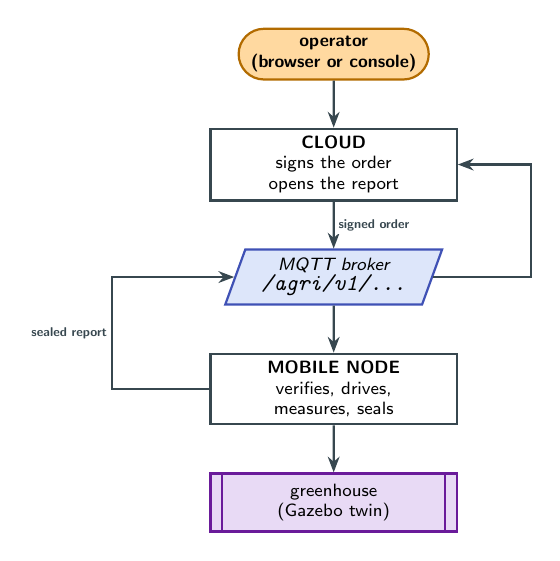
\begin{tikzpicture}[fcchain, scale=0.92, transform shape]
  \node[fcterm]                                (op)  {operator\\(browser or console)};
  \node[fcproc, below=of op]                   (cl)  {\textbf{CLOUD}\\signs the order\\opens the report};
  \node[fcio,   below=of cl]                   (br)  {MQTT broker\\\topicname{agri/v1/\ldots}};
  \node[fcproc, below=of br]                   (rb)  {\textbf{MOBILE NODE}\\verifies, drives,\\measures, seals};
  \node[fcsub,  below=of rb]                   (gz)  {greenhouse\\(Gazebo twin)};

  \draw[fcline] (op) -- (cl);
  \draw[fcline] (cl) -- node[fclab,right]{signed order} (br);
  \draw[fcline] (br) -- node[fclab,right]{} (rb);
  \draw[fcline] (rb) -- (gz);
  \draw[fcline] (rb.west) -- ++(-1.35,0) |- node[fclab,left,pos=0.25]{sealed report} (br.west);
  \draw[fcline] (br.east) -- ++(1.35,0) |- (cl.east);
\end{tikzpicture}
\caption{\phaseC{} at a glance. The two processes never address each
other: the broker is the only endpoint either configures. The order is
\emph{signed} and readable; the report is \emph{sealed} and is not
(Sec.~\ref{sec:phaseC_security}).}
\label{fig:phaseC_arch}
\end{figure}

\subsection{What is measured, and by what}

The robot reports five environmental quantities per station ---
temperature, relative humidity, illuminance, CO\textsubscript{2} and
soil pH --- together with its own pose and velocity at the instant of
reading.

\textbf{These readings are synthesised, and the system says so out
loud.} Gazebo models no soil chemistry and no CO\textsubscript{2}
diffusion; there is nothing in the simulator to sample. They are
generated by \filename{agri/sensors.py} as a smooth spatial field with a
diurnal component and four deliberately planted anomalies, and the robot
node prints this at startup on every run:

\begin{lstlisting}[style=bash]
agri_robot youbot-01: keys in .../keys, readings are
SYNTHESISED by agri.sensors (Gazebo has no probes)
\end{lstlisting}

The honest description of what \phaseC{} validates is therefore: the
\emph{chain} is real --- the driving, the alignment, the encoding, the
cryptography, the transport, the storage, the refusals --- and the
\emph{numbers entering it} are a stand-in for a probe that does not
exist in simulation. Substituting a real sensor changes one function and
nothing else, which is exactly why that function is isolated.

The anomalies exist so the chain can be shown to carry information and
not merely bytes: a dry patch at \station{P2,4}, elevated
CO\textsubscript{2} at \station{P3,7}, and a pH excursion at
\station{P1,2}. Each survives the QR encoding, the seal, the transport
and the store, and appears flagged on the dashboard --- which is
visible in the campaign log of Sec.~\ref{sec:results}, where
\station{P2,4R} arrives at \measured{47.8\%} humidity against a
\measured{$\approx$70\%} field, and \station{P3,7R} at
\measured{1070~ppm} against \measured{$\approx$550~ppm}.

\subsection{Reading order}

The remaining \phaseC{} sections follow the path of one measurement,
from the coordinate that defines where it is taken to the check that
proves it arrived intact:

\begin{itemize}[leftmargin=*,itemsep=1pt,topsep=2pt]
  \item Sec.~\ref{sec:phaseC_catalogue} --- the 48 stations, and why the
        world is generated from them rather than described twice.
  \item Sec.~\ref{sec:phaseC_nav} --- deterministic navigation, and the
        case for deleting the planner.
  \item Sec.~\ref{sec:phaseC_align} --- closing the last centimetres on
        a painted mark with a downward camera.
  \item Sec.~\ref{sec:phaseC_measurement} --- the reading, the QR code,
        the photograph.
  \item Sec.~\ref{sec:phaseC_security} --- what is signed, what is
        encrypted, and why those are different questions.
  \item Sec.~\ref{sec:phaseC_protocol} --- the MQTT contract and the
        multi-node topic layout.
  \item Sec.~\ref{sec:phaseC_cloud} --- the Cloud, the store, the
        dashboard, and the three timestamps a reading carries.
  \item Sec.~\ref{sec:phaseC_route} --- route optimisation and the
        energy budget.
  \item Sec.~\ref{sec:phaseC_regression} --- the 384-check pre-flight
        suite.
\end{itemize}

% =====================================================================
%  Phase C --- The station catalogue and the generated world
%  SCOPE: one source of coordinates; the world is built from it.
% =====================================================================
\section{The Station Catalogue and the Generated World}
\label{sec:phaseC_catalogue}

\subsection{Forty-eight stations}

The \phaseB{} greenhouse (Sec.~\ref{sec:phaseB_twin}) is
$9.90 \times 4.90$~m internally, with three planting gutters 0.40~m wide
centred at $y = -1.20$, $0.00$ and $+1.20$~m, and eight plants per row
spaced 0.90~m apart from $x = -3.15$~m. \phaseC{} adds a
\emph{measurement station} on each side of each plant: 3 rows
$\times$ 8 plants $\times$ 2 sides $= 48$, labelled \station{Pi,jR} and
\station{Pi,jL}.

A station is a point on the floor where the robot's sensor head must
stand, offset \SI{0.55}{m} across the row from the plant centre. The
label grammar is deliberately the one an agronomist would speak:
\station{P2,5} names a \emph{plant} and expands to both of its stations;
\station{P2,5R} names one side. Expansion happens on the Cloud, before
the order is signed, so the robot never interprets a wildcard --- a
robot that expanded \texttt{ALL} itself would silently disagree with the
Cloud the day the greenhouse gained a row.

\subsection{The decision that shapes everything else}

Three programs need these coordinates and must not disagree: the world
generator that paints the marks, the robot that drives onto them, and
the dashboard that draws them.

The obvious construction is to type the numbers into the world file and
again into the robot. That is how a mark ends up painted at $y=-1.70$
and driven to at $y=-1.65$, with the robot then reporting that it is
``on'' a mark it is 5~cm away from and nothing anywhere to catch it.
\phaseC{} therefore inverts the dependency: the numbers exist once, in
\filename{agri/catalogue.py}, and \textbf{the greenhouse is generated
from them}.

\begin{lstlisting}[style=bash]
python3 -m agri.world.make_world   # reads the Phase B scene,
                                   # paints 48 marks from the catalogue
python3 -m agri.world.make_robot   # adds the boom and floor camera
\end{lstlisting}

The regression suite closes the loop in both directions: it reads the
plant positions back out of the \phaseB{} world and asserts the
catalogue still agrees with them, and it parses the generated SDF and
asserts every painted mark is where the catalogue says. Neither the
greenhouse nor the robot can drift from the map without a check going
red (Sec.~\ref{sec:phaseC_regression}).

The generator also refuses to run twice over its own output, because
re-painting an already-painted world produces 96 marks and a scene that
looks subtly wrong rather than obviously broken.

\subsection{Two geometric constraints that fixed the numbers}

Two constants were not chosen by preference. They are reported here
because both were got wrong first, and because each is the kind of value
that looks arbitrary until the reason is written down.

\paragraph{Station reach, \SI{0.55}{m}} An inner aisle is only 0.80~m
wide between two gutter edges. The natural design --- turn the base to
face the plant --- points the chassis' long axis across that aisle,
putting 0.29~m of half-length toward the gutter instead of 0.19~m of
half-width, and the two stations sharing an inner aisle then cannot both
fit with usable margin. The first attempt left \SI{1}{cm}.

\phaseC{} keeps the base \emph{along} the aisle and lets the existing
pan head look sideways, which is what the head is for. That converts
0.29 into 0.19 and buys back 0.20~m. At a reach of \SI{0.55}{m}, the
tightest of all 48 stations (\station{P2,1R}) then clears every gutter
and wall by \measured{\SI{0.16}{m}}, and the suite asserts that bound on
every run.

\paragraph{Cross arm, \SI{0.04}{m}} The price of the above is that the
two stations sharing an inner aisle sit only \SI{0.10}{m} apart, at the
same $x$. Their $y$-arms therefore lie on one line. Any arm longer than
\SI{0.05}{m} makes the two painted crosses touch, and a blob detector
then sees \emph{one} marker straddling both --- it would centre the
robot on the midpoint, \SI{0.05}{m} from either station, and file the
visit under whichever label it guessed.

\SI{0.04}{m} leaves a \SI{0.02}{m} gap, about ten pixels for the floor
camera. An earlier version used \SI{0.09}{m} and carried a comment
asserting the crosses did not merge; rendering the pair and running the
detector over it is what showed the comment was wrong. The suite now
renders adjacent pairs and asserts the nearer mark wins at three
different offsets.

\subsection{Why the marks are painted at all}

\SI{0.10}{m} is inside the error a drifting odometric estimate
accumulates in a single lap of this greenhouse. Driving to a station on
odometry alone is therefore not merely imprecise --- it is capable of
parking the robot closer to the neighbouring station than to the one it
is about to file a reading under, which corrupts the \emph{label} rather
than the value. The painted marks exist so that the final approach can
be closed visually against a physical feature of the building, which is
the subject of Sec.~\ref{sec:phaseC_align}.

% =====================================================================
%  Phase C --- Deterministic navigation
%  SCOPE: the free-space decomposition, the three-leg route, the brake.
% =====================================================================
\section{Deterministic Navigation}
\label{sec:phaseC_nav}

\subsection{Autonomous, but not exploratory}

This section states plainly what \phaseC{} navigation is, because the
distinction is easy to lose and a reader may reasonably assume that
removing SLAM removed autonomy.

The robot in \phaseC{} is fully autonomous in the control sense: it
receives a list of station labels and nothing else, and it decides its
own route, drives itself in closed loop, brakes on its own sensor
evidence, and corrects its own final position against what it sees.
There is no teleoperation and no trajectory replay.

What it does \emph{not} do is discover. It never builds a map, never
decides where to go next based on what it found, and never searches for
a path. It cannot, because the question does not arise: the map is a
catalogue that predates the robot (Sec.~\ref{sec:phaseC_catalogue}), and
the order names the stations explicitly. The autonomy that remains is
\emph{deterministic} rather than \emph{exploratory}, and the difference
is worth naming precisely rather than describing as ``less''.

\subsection{The free space, decomposed once}

The greenhouse free space is not a general planning problem. It is four
corridors joined at both ends, and \filename{agri/aisles.py} derives
that decomposition from the wall and gutter coordinates rather than
declaring it:

\begin{table}[!t]
\caption{The free bands, derived from the catalogue. Each is an interval
of the robot centre line in $y$; every station lies in exactly one.}
\label{tab:bands}
\centering\footnotesize
\begin{tabular}{@{}clc@{}}
\toprule
band & $y$ interval (m) & stations \\
\midrule
0 & $[-2.45,\; -1.40]$ & \station{P1,*R} \hfill 8 \\
1 & $[-1.00,\; -0.20]$ & \station{P1,*L}, \station{P2,*R} \hfill 16 \\
2 & $[+0.20,\; +1.00]$ & \station{P2,*L}, \station{P3,*R} \hfill 16 \\
3 & $[+1.40,\; +2.45]$ & \station{P3,*L} \hfill 8 \\
\bottomrule
\end{tabular}
\end{table}

At each end, past the \SI{8.0}{m} gutters, lies a \emph{headland} that
joins all four bands. A route is therefore at most three legs --- out to
a headland, across to the target band, in to the station --- and
choosing between the two headlands is a comparison of two numbers, not a
search:

\begin{lstlisting}[style=python]
def route(sx, sy, tx, ty):
    here, there = band(sy), band(ty)
    if here is not None and here == there:
        return [(tx, ty)]                 # one leg
    end = min(HEADLANDS,
              key=lambda e: abs(sx - e) + abs(e - tx))
    return [(end, sy), (end, ty), (tx, ty)]
\end{lstlisting}

\paragraph{Why no planner} A$^\star$ over an occupancy grid would spend
a millisecond rediscovering Table~\ref{tab:bands}, and would then be
free to discover something \emph{else} on a day when the grid was subtly
wrong. That is not a hypothetical: it is what \phaseA{} did in a
\SI{0.16}{m} clearance (Sec.~\ref{sec:phaseA_planning}). A closed-form
route cannot produce a novel answer, which in a corridor with
\SI{0.16}{m} of margin is a feature.

The cost of that choice is that the geometry must be right, so it is
verified exhaustively rather than argued: the suite sweeps
\textbf{all 2\,256 station-to-station routes}, plus every route out of
the dock, and asserts the robot's rectangle never comes within
\SI{0.08}{m} of a gutter or a wall on any leg of any of them. That runs
in about a second and needs nothing installed.

\subsection{The asymmetry that a symmetric model hides}

The two headlands are \textbf{not} at symmetric coordinates:
$x_{\text{west}} = \measured{-4.08}$~m and
$x_{\text{east}} = \measured{+4.87}$~m. The robot is not symmetric --- a
\SI{0.50}{m} sensor boom points $+x$ and \SI{0.29}{m} of chassis trails
behind --- so at the west end the sensor point leads and must stop short
of the gutters, while at the east end the sensor point goes deep and the
\emph{tail} must clear them. The footprint ends up centred in the
\SI{0.95}{m} gap either way, with \SI{0.08}{m} of margin at each end.

An earlier version used one number for both. Going east, that left the
chassis lying alongside the gutters while the robot strafed across the
greenhouse --- straight through them. \textbf{Nothing would have
reported it.} This robot carries no collision geometry, so driving
through a gutter produces no contact, no warning and no complaint, only
a recording that cannot be shown to anyone. It was caught by the
clearance sweep above, which is the entire reason that function exists.

\subsection{The brake, and what it must ignore}

The route is geometric; the lidar is not. During every leg the robot
tests each return against the corridor it is about to sweep. Two design
choices carry the section.

\paragraph{A corridor, not a cone} A $\pm35\degree$ cone was the first
version, and it stopped the robot dead in every aisle: at \SI{0.35}{m}
of lateral clearance, a gutter wall the robot is driving \emph{parallel}
to sits well inside a $35\degree$ cone, so the brake fired on the very
thing the route was designed to pass. A corridor asks the only question
that matters --- is this in the way? --- and a wall you are driving
alongside is not in the way.

The corridor's edges are the extreme projections of the robot's own four
corners onto the axis across the direction of travel. For a symmetric
robot a half-width would do; with a \SI{0.50}{m} boom in front and
\SI{0.29}{m} of chassis behind, a \emph{strafing} robot sweeps
\SI{0.79}{m} and not centred on the base.

\paragraph{The building is not an obstacle} The brake exists for things
that should not be there. The walls and the gutters should be there,
they are in the catalogue, and the sweep above has already proved every
route clears them. Braking for them is not caution; it is refusing to
move --- and it produced two failures that looked entirely different:

\begin{itemize}[leftmargin=*,itemsep=1pt,topsep=2pt]
  \item \emph{Every leg to a headland stopped.} The robot must back its
        tail to within \SI{0.08}{m} of the end wall to fit the
        \SI{0.95}{m} gap; the brake wanted \SI{0.35}{m} of clear floor
        and refused \SI{0.27}{m} short. The mission logged ``something
        is in the aisle''. Something was: the building.
  \item \emph{A leg that shifts sideways while advancing} ---
        \SI{0.10}{m} across while travelling \SI{0.66}{m} along, which
        is exactly what moving between the two stations of an inner
        aisle looks like --- tilts the swept corridor by $8.6\degree$
        and swings it onto the gutter the robot is driving \emph{beside}.
        Same wall, different geometry, same wrong answer.
\end{itemize}

Both are resolved by projecting each return into world coordinates and
discarding it when it falls within \SI{0.12}{m} of catalogued structure.
A return \emph{inside} the robot's own outline is discarded too: the
lidar sits within the chassis and sees the camera pedestal and the mast
at \SI{0.12}{m} and \SI{0.22}{m} ahead, which a raw range test brakes
for permanently, from the first metre.

The suite pins both behaviours from opposite sides --- a gutter being
driven past does not stop the robot, an object genuinely ahead does, and
no station stands on a point the brake would ignore --- so neither fix
can be undone by loosening the other.

% =====================================================================
%  Phase C --- Visual alignment on the painted mark
%  SCOPE: the downward camera, the detector, the bounded correction.
% =====================================================================
\section{Closing the Last Centimetres}
\label{sec:phaseC_align}

\subsection{Why odometry is not enough here}

Sec.~\ref{sec:phaseC_catalogue} established the constraint: two stations
sharing an inner aisle are \SI{0.10}{m} apart. Sec.~\ref{sec:slam}
established the measurement: uncalibrated odometry on this platform
diverges past \SI{10}{m} over a mission, and even calibrated it holds
only \measured{\SI{0.20}{m}}.

\SI{0.20}{m} is twice the station spacing. The failure this produces is
not an imprecise reading --- it is a \emph{correctly measured value
filed under the wrong label}, which is worse, because nothing downstream
can detect it. A campaign so corrupted looks complete.

\subsection{The sensor point is the camera, not the base}

\phaseC{} adds a downward camera on a short boom over the front bumper,
and makes \emph{that} point the one a station names.

A robot that has a body cannot see the floor under its own middle --- the
chassis is in the way --- so a mark under the centre can be driven to but
never verified. Putting the reference point under a downward camera makes
``the mark is in the middle of the picture'' and ``the sensor is on the
mark'' the same statement, with no lever arm whose sign can be got wrong.

\SI{0.50}{m} is the smallest offset that also keeps the camera mast out
of the downward view cone: the mast reaches $x = 0.27$~m at \SI{0.45}{m}
height, and a camera at \SI{0.50}{m} sees the floor from $x = 0.27$~m
outwards, so no ray crosses it. Two consequences follow and are stated
once: the base centre stands \SI{0.50}{m} back along the aisle from the
station, and \textbf{every pose in every report is the sensor point},
not \texttt{base\_link}.

\subsection{Detecting a cross, and refusing a blob}

The detector (\filename{agri/vision.py}) is a red-dominance threshold
followed by a connected-component pass, with three refusals that matter
more than the detection itself:

\begin{itemize}[leftmargin=*,itemsep=1pt,topsep=2pt]
  \item \textbf{A solid blob is not a cross.} A cross fills
        \measured{$\approx$44\%} of its own bounding box; a filled square
        fills 100\%. Rejecting on fill ratio stops the robot from
        centring on a red object that is not a station mark. The
        accepted band is deliberately wide, because the exact ratio
        moves with the arm and thickness constants, and a detector that
        needed retuning whenever the paint changed would be retuned
        wrong.
  \item \textbf{A clipped cross is refused, not averaged.} A mark half
        out of frame has a centroid that is not its centre. Averaging it
        yields a confident correction in the wrong direction.
  \item \textbf{The nearer of two marks wins.} With a neighbour
        \SI{0.10}{m} away the frame can contain both. The suite asserts
        the nearer one is selected at three different offsets, including
        one where the robot starts closer to the neighbour.
\end{itemize}

The threshold itself needs no tuning: the aisle paint is dark green
$(38, 64, 54)$ and the gutters are near white, so a factor-1.6 dominance
test separates the marker from both by a wide margin. This is a
consequence of the world being generated (Sec.~\ref{sec:phaseC_catalogue})
--- the detector and the paint come from the same file.

\subsection{The correction is bounded, and the bound is not a preference}

The visual correction is capped at \measured{\SI{0.04}{m}} per station.

The reasoning is the same \SI{0.10}{m} that drove the arm length: a
correction larger than \SI{0.05}{m} could leave the robot nearer the
\emph{neighbouring} station than the one it is about to file under. The
Cloud would then reject the report --- correctly --- for a reason with
nothing to do with the plant. \SI{0.04}{m} keeps a clear margin under
that bound and is still four times the residual the odometric approach
leaves behind.

The robot makes at most four correction attempts, stopping when the
residual falls below \SI{0.008}{m}.

\subsection{What happens when the camera cannot see}

The mark can be missing, occluded, or outside the frame. \phaseC{} does
not treat that as a mission failure and does not silently pretend it
did not happen. The robot parks on odometry alone, says so in the log,
and \textbf{increments a counter that travels with the mission report}:

\begin{lstlisting}[style=bash]
mission 788081147cfd finished in 601 s, floor camera
used at 48 station(s), unavailable at 0
\end{lstlisting}

That line is the honest form of the accuracy claim. Rather than
asserting a parking error the simulator cannot independently confirm,
the system reports \emph{how many of the visits were closed visually}
and lets the reader judge. In the reference campaign of
Sec.~\ref{sec:results} the camera resolved its mark at
\measured{48 of 48} stations, and at \measured{52 of 52} across the full
session including the four single-station re-measurements.

Every report additionally carries its own \param{parking\_error\_m}, and
the Cloud checks it against the catalogue independently of what the
robot believed --- so a visit filed under the wrong label is detectable
after the fact, from the stored record alone.

% =====================================================================
%  Phase C --- The measurement, the QR code, the photograph
% =====================================================================
\section{The Measurement and Its Encodings}
\label{sec:phaseC_measurement}

\subsection{What one visit produces}

A visit yields three artefacts, and they are deliberately redundant:

\begin{enumerate}[leftmargin=*,itemsep=1pt,topsep=2pt]
  \item the five readings as numbers, with the station label, a UTC
        timestamp, and the robot's pose and velocity;
  \item the same content as a \textbf{QR code image};
  \item a \textbf{photograph} of the plant, taken by the pan camera
        turned toward the row.
\end{enumerate}

\subsection{The robot reports on itself, not only on the plant}

Every measurement carries the robot's own pose and its three velocity
components at the instant of reading. This is not telemetry padding.

A reading taken while the platform is still rolling is a reading taken
\emph{somewhere between two places}. Because the velocity travels inside
the sealed payload and inside the QR code, that condition is detectable
afterwards, from the archived record, by someone who was not present.
The velocity is read \emph{after} the sensors rather than before, for
the same reason: it is the speed at the moment of the reading that
qualifies the reading.

The speed is transmitted as the magnitude alongside the components, and
the suite asserts it really is the magnitude and not a component --- a
substitution that would look plausible in every log and be wrong for
every strafing move.

\subsection{The QR code, and why it is not decoration}

The payload is a single pipe-separated line, human-legible when scanned:

\begin{lstlisting}[style=bash]
AGRI1|P1,1R|2026-08-08T19:23:27Z|t=21.4|rh=76.2
|lux=19272|co2=552|ph=6.84|x=-3.146|y=-1.745
|yaw=180.0|vx=-0.003|vy=0.007|w=0.000
\end{lstlisting}

\measured{128 characters}, which a phone camera reads off a screen and
returns as the original numbers. Three properties are asserted by the
suite over all 48 station codes:

\begin{itemize}[leftmargin=*,itemsep=1pt,topsep=2pt]
  \item every code encodes and decodes again;
  \item the decoded text round-trips through the JSON
        \emph{character for character};
  \item a payload from another system is refused rather than
        misparsed --- \texttt{HELLO|P2,5R} is rejected with
        ``not an AGRI1 payload'', as is an unknown quantity key.
\end{itemize}

The Cloud re-reads every QR image it receives and checks the decoded
numbers against the ones that travelled beside it in the JSON. This is
the project's only \emph{end-to-end} content check: it would catch a
corrupted image, a mismatched pairing, and an encoder that silently
rounded. Two decoders are installed because OpenCV fails to locate 2 of
the 48 station codes while zxing-cpp reads all 48; either alone works,
and the tests run against both.

\subsection{The photograph}

The pan head turns toward the plant using the station's stored bearing,
so the same station works whichever way along the aisle the robot is
travelling --- storing a fixed robot yaw instead would silently assume a
direction and make half the visits look the wrong way. The suite asserts
the head pans $+90\degree$ driving east at an \station{R} station,
$-90\degree$ driving west at the same one, and the opposite for
\station{L}.

The image is JPEG-compressed and travels base64-encoded inside the
sealed envelope. The Cloud writes it back out as a file and keeps only
the path in the record (Sec.~\ref{sec:phaseC_cloud}).

\subsection{The synthesised field}

As stated in Sec.~\ref{sec:phaseC}, the five readings are generated
rather than sensed. The field is not noise: it is smooth in space, so
neighbouring plants correlate; it is deterministic, so the same station
reads the same twice; it carries a diurnal component driven by simulator
time; and it contains the three planted anomalies of
Table~\ref{tab:anomalies}.

\begin{table}[!t]
\caption{The planted anomalies. Each is asserted by the suite to stand
out from its neighbourhood, so a change to the field cannot silently
flatten the signal the dashboard exists to show.}
\label{tab:anomalies}
\centering\footnotesize
\begin{tabular}{@{}llr@{}}
\toprule
stations & quantity & offset \\
\midrule
\station{P2,4R} / \station{P2,4L} & humidity        & $-22.0$ / $-20.0$ \%RH \\
\station{P3,7R} / \station{P3,7L} & CO\textsubscript{2} & $+480$ / $+455$ ppm \\
\station{P1,2R} / \station{P1,2L} & pH              & $+1.35$ / $+1.30$ \\
\bottomrule
\end{tabular}
\end{table}

Both stations of an affected plant are perturbed, by slightly different
amounts. A single-sided anomaly would be indistinguishable from a
sensor fault, and identical values on both sides would be
indistinguishable from a constant --- neither would exercise the
comparison the dashboard invites the operator to make.

% =====================================================================
%  Phase C --- Cryptography: what is signed, what is sealed, and why
% =====================================================================
\section{Authenticity and Confidentiality}
\label{sec:phaseC_security}

\subsection{Two different questions}

Habit says encrypt everything. Resisting that habit is what makes this
part of the design legible, so the two directions are treated
separately and the reasoning is written down.

\paragraph{Cloud $\rightarrow$ robot: signed, not encrypted} A request
says ``measure \station{P2,5R}''. That is not a secret. But issuing one
drives a robot around a greenhouse, and anyone who can reach the broker
can publish on the topic. The property that matters is therefore
\emph{authenticity}, not confidentiality. Requests carry an ECDSA-P256
signature over the canonical JSON; the robot refuses an unsigned request
and refuses one signed by the wrong key.

\paragraph{Robot $\rightarrow$ Cloud: sealed and signed} A report
contains the agronomic state of a commercial crop and a photograph of
it. It needs confidentiality \emph{and} origin, and gets both.

\subsection{The envelope}

Reports are sealed with ECIES over SECP256R1: an ephemeral key pair per
message, ECDH against the Cloud's public key, HKDF-SHA256 to derive the
content key, and AES-256-GCM for the payload. The ciphertext is then
signed with the robot's long-term ECDSA-P256 key. The complete wire
message is:

\begin{lstlisting}[style=bash]
{"schema":"agri-cloud/v1", "kind":"sealed",
 "robot":"youbot-01", "request_id":"...",
 "sent_at":"2026-08-08T19:23:27Z",
 "sealed": {
   "alg":  "ECIES-P256-HKDF-SHA256-AES256GCM",
   "epk":  "-----BEGIN PUBLIC KEY-----...",
   "nonce":"UgoQGAyNp7LauuRB",
   "ciphertext":"5k2ZWwLpBQVmV61fDxBg39Xy...",
   "sig":  "MEUCIGmZLjCjPHsyhdx97dGKKhmk..." }}
\end{lstlisting}

The routing metadata --- who sent it, for which request, when --- stays
in clear, because the broker and the operator need it to route and to
diagnose, and none of it is the measurement. The readings, the pose, the
QR image and the photograph are all inside the ciphertext.

\subsection{Sign-then-encrypt, or encrypt-then-sign}

The signature is over the \emph{ciphertext}. This is deliberate: it lets
the Cloud reject a forged message without first performing a private-key
operation on attacker-chosen input, and it means a tampered ciphertext
is detected by the cheap check rather than by AES-GCM's authentication
tag alone.

The suite pins six properties of this construction, and four of them are
refusals:

\begin{table}[!t]
\caption{Cryptographic properties asserted on every run. The refusals
matter more than the round trip: a system that accepts everything also
round-trips perfectly.}
\label{tab:crypto}
\centering\footnotesize
\begin{tabular}{@{}p{0.50\columnwidth}p{0.40\columnwidth}@{}}
\toprule
property & verdict \\
\midrule
a sealed payload round-trips              & \ok{accepted} \\
the plaintext is absent from the envelope & \ok{confirmed} \\
the wrong recipient key cannot open it    & \bad{refused} \\
a forged sender is rejected               & \bad{refused} \\
stripping the signature does not bypass the check & \bad{refused} \\
one flipped bit is detected               & \bad{refused} \\
the same plaintext seals differently every time & \ok{confirmed} \\
a rewritten target breaks the request signature & \bad{refused} \\
\bottomrule
\end{tabular}
\end{table}

The third-from-last matters more than it looks: an ephemeral key per
message means two identical readings produce two unrelated ciphertexts,
so an observer cannot tell that a station was measured twice with the
same result.

\subsection{Key custody, and the refusal that protects it}

The Cloud is meant to run on a different machine from the robot. That
intent is enforced rather than documented:

\begin{itemize}[leftmargin=*,itemsep=1pt,topsep=2pt]
  \item An \textbf{empty} key directory is bootstrapped with both pairs,
        so a first run on one machine works with no ceremony.
  \item A \textbf{populated} key directory is never bootstrapped behind
        the operator's back.
  \item \textbf{Neither side ever generates the other side's key.} The
        Cloud will not invent a robot identity; the robot will not
        invent a Cloud identity.
\end{itemize}

That last rule is the one that earns its place. Without it, a Cloud
started on a fresh machine with a forgotten key copy would generate a
robot public key of its own, and then reject every report from the real
robot --- with a valid signature failure, forever, and no indication
that the cause was a missing file. Instead it refuses to start and names
the file:

\begin{lstlisting}[style=bash]
/path/forgot/cloud_public.pem is missing.
\end{lstlisting}

The suite exercises the whole two-machine story: bootstrap an empty
directory, copy only the public keys to a second directory, start a
robot there, and assert that it runs \emph{and} that it does not hold
the Cloud's private key.

\subsection{Refusals are counted, not dropped}

A report that fails to open is not discarded silently. It is counted,
its reason is kept, and the dashboard displays it under
\textsc{rejected}. A pipeline that hides its rejections is a pipeline
that will one day be receiving nothing and look perfectly healthy.

In the reference campaign the panel read \emph{``nothing refused ---
every report verified''} across all \measured{48} reports, which is the
statement worth making: not that the cryptography was exercised, but
that it was exercised and nothing failed.

% =====================================================================
%  Phase C --- The MQTT contract
% =====================================================================
\section{The Transport Contract}
\label{sec:phaseC_protocol}

\subsection{Why MQTT and not HTTP}

The Cloud must be able to reach the robot, not only the other way round.
With HTTP the robot would have to poll for work; with MQTT it subscribes
once and the broker pushes. The broker is also the only endpoint either
side configures: neither has to know the other's address, and either can
restart without the other noticing. That is the property that makes
``the robot is a node on a network'' an architectural fact rather than a
turn of phrase.

It is additionally the protocol the rest of the agricultural-IoT world
speaks, so the same robot could report to a different back end without a
line changing in \filename{agri/protocol.py}.

\subsection{Topics, namespaced by node}

\begin{table}[!t]
\caption{The topic contract. Robot-to-Cloud topics are namespaced per
node; the Cloud subscribes with MQTT wildcards.}
\label{tab:topics}
\centering\footnotesize
\begin{tabular}{@{}llp{0.30\columnwidth}@{}}
\toprule
topic & direction & payload \\
\midrule
\topicname{agri/v1/request}              & Cloud $\rightarrow$ all & signed, readable \\
\topicname{agri/v1/ack/<node>}           & node $\rightarrow$ Cloud & plain progress \\
\topicname{agri/v1/report/<node>}        & node $\rightarrow$ Cloud & sealed \\
\topicname{agri/v1/status/<node>}        & node $\rightarrow$ Cloud & plain, retained \\
\bottomrule
\end{tabular}
\end{table}

Requests stay on a \emph{flat} topic because a request addresses the
fleet, not a specific node. Everything a node says is namespaced by its
own identifier, and the Cloud subscribes with \texttt{+} to hear all of
them, keeping nodes in a dictionary rather than a single variable. There
is one mobile node today; the layout is what stops adding a second from
being a protocol change.

\subsection{Node kinds}

Every status message carries a \param{node\_kind} field:
\texttt{"mobile"} for a robot that drives between stations,
\texttt{"fixed"} for a stationary microcontroller bolted to a post. The
field is carried now, with one mobile node and no fixed ones, so that
adding fixed sensors later does not change the protocol --- and so that
the priority rule it exists for (prefer the mobile reading when a robot
is parked at a station a fixed node also covers) has somewhere to live.

\subsection{Three choices that were not defaults}

\paragraph{QoS 1, not 0 or 2} Zero would drop a request while the robot
is mid-reconnect. Two costs a four-way handshake for no benefit here,
because the request identifier already makes a repeat harmless --- and
the store deduplicates on (label, timestamp, robot), which catches
exactly the case QoS~1 permits and nothing else.

\paragraph{Status is retained; nothing else is} A dashboard opened at
any moment should immediately know whether the robot is there, and MQTT's
retained flag gives precisely that. Retaining \emph{reports} instead
would mean every reconnecting client re-receives the last measurement and
files it again, which is how duplicates appear in a store that has no
reason to have any.

\paragraph{A last will} If the robot process dies, the broker tells the
Cloud on the node's own status topic. A dashboard that shows a robot as
online because nobody said otherwise is worse than one that shows
nothing.

\subsection{Two failures the transport layer had to survive}

Both were observed, and both are now pinned by the suite.

\paragraph{A broker that is not up yet} The robot node originally exited
when it could not connect, which made the launch order of two terminals
load-bearing --- start the simulation before the broker and the robot was
simply gone, with the failure scrolled off the top of a 140-line startup
log. It now waits, retries with a bounded backoff, re-subscribes on
\emph{every} connect rather than only the first, says so when the broker
goes away, and complains on the wall clock if none ever appears.

\paragraph{An exception inside an MQTT callback} \texttt{paho} does not
guard its callbacks: an exception raised inside one kills its network
thread. The observed symptom was a robot that looked perfectly healthy
--- its status timer kept publishing, because that runs on a different
thread --- while every request the Cloud sent was delivered to a client
that was no longer reading. Forty minutes of a robot that would not move
and a log that said nothing.

The cause was the status callback asking the driver for a pose before
the simulator had published any odometry. Two rules came out of it and
are asserted statically: no MQTT callback may let an exception escape,
and \texttt{status()} must never raise even with no odometry at all --- a
status with no position is still worth sending, because ``I am here and
I am connected'' is exactly what the Cloud needs at that instant.

% =====================================================================
%  Phase C --- The Cloud: store, timestamps, dashboard
% =====================================================================
\section{The Cloud}
\label{sec:phaseC_cloud}

\subsection{One process, two faces}

The Cloud is deliberately a single process presenting two interfaces: an
MQTT client that talks to robots, and an HTTP server that talks to the
operator. A third interface, a console on the main thread, is where
orders are actually typed --- the operator's seat is in the process that
holds the private key.

\paragraph{No web framework} The API has five endpoints and
\texttt{http.server} is in the standard library. A framework would add a
dependency, a version to pin and a deployment story, and would not make
any of the five shorter. The one thing it would buy --- production-grade
concurrency --- is not needed by a dashboard with one operator, and
pretending otherwise would be the kind of choice that looks like
engineering and is not.

\subsection{Storage: JSON Lines, not a database}

The brief asks for storage in a file of appropriate format. Appropriate
here means openable by a human, appendable without rewriting, and
diffable --- which is JSON Lines: one visit per line, append-only, plus
the images written out as real files, plus a CSV rebuilt on demand.

\begin{lstlisting}[style=bash]
store/
  measurements.jsonl        append-only, one visit per line
  photos/P2,5R/2026....jpg  the photograph, as sent
  qr/P2,5R/2026....png      the QR code, as sent
  measurements.csv          rebuilt on export
  requests.csv              one row per order
\end{lstlisting}

A database would be defensible and is what a production system would
use. It would also mean the evidence for every number in this report
lives inside a binary file nobody can inspect during a demonstration.
For a system whose entire claim is that the data arrived intact, being
able to open the file and read the line is worth more than query speed
over a few thousand rows.

The images come back out of the JSON because leaving them there would
make the file unreadable --- a 6~kB blob per line --- and would mean the
only way to look at a photograph is to write a program. Extracted, the
line stays about 400 bytes and legible.

One corrupt line does not cost the campaign: the loader names the line
it skipped and keeps the rest, because a truncated final line is what a
kill during a write looks like and it is recoverable.

\subsection{Three timestamps, because there are three moments}

A reading has three distinct times, and the system originally kept one.
The only honest answer to ``how long did that sweep take'' was then to
watch a clock while it ran.

\begin{table}[!t]
\caption{The three moments a stored reading carries, each on the clock
of the machine that owns it. End-to-end latency is derivable from the
stored line alone.}
\label{tab:timestamps}
\centering\footnotesize
\begin{tabular}{@{}ll@{}}
\toprule
field & the moment it records \\
\midrule
\param{request\_issued\_at} & the Cloud signed the order \\
\param{measured\_at}        & the robot read the plant \\
\param{received\_at}        & the Cloud filed the report \\
\param{latency\_s}          & derived: issued $\rightarrow$ received \\
\bottomrule
\end{tabular}
\end{table}

The column \param{timestamp} was removed rather than redefined, and the
suite asserts it is gone --- with three moments in play, a field called
``timestamp'' is a question, not an answer.

Orders are tracked in parallel in \filename{requests.csv}, with
\param{issued\_at}, \param{completed\_at} and \param{elapsed\_s}. A
mission that ends \emph{without} filing every report still ends: the
record closes on the terminal acknowledgement, so an abandoned sweep
reports how long it ran before giving up rather than showing as running
forever. The dashboard distinguishes the two verbs --- ``done'' versus
``gave up'' --- because the same numbers under the same word would
report a failure as a success in the one place an operator looks for the
answer.

\subsection{The dashboard}

The dashboard is a single page with no build step and no framework,
polling \texttt{/api/state} every two seconds. It shows the greenhouse
as a scale map with all 48 stations, the readings of the selected
quantity, the plant photograph and QR image, live request progress, and
the rejection panel.

Two problems in it are worth recording because both are geometric rather
than aesthetic:

\begin{itemize}[leftmargin=*,itemsep=1pt,topsep=2pt]
  \item \textbf{The two stations of an inner aisle collide when drawn.}
        At \SI{0.10}{m} apart their marks touch at map scale. Each value
        chip is pushed away from its own row and joined to its mark by a
        stem, and the suite asserts the plain rendering really does
        collide and the corrected one does not --- so the fix cannot be
        removed by someone who thinks it is decoration.
  \item \textbf{Text inherits the map's flip.} The SVG applies a
        $y$-negating transform so that $+y$ is north; every text element
        must counter-flip it or read mirrored. That counter-flip is
        written once, in a helper, and the suite asserts it is not
        open-coded per call site.
\end{itemize}

\paragraph{Access control} The dashboard API is protected by a random
token printed at startup. \texttt{/media/} is behind the same token:
photographs, QR images and the CSV export are measurements, so they sit
behind the same gate as the API that describes them.

The token is offered once, in the URL, and the server's first act is to
get rid of it: it sets an \texttt{HttpOnly; SameSite=Strict} cookie and
redirects to the same page with the query string stripped. A credential
that authorises driving the robot has no business living in the address
bar, the browser history, the \texttt{Referer} of every outbound link
and any proxy log in between. Repeated wrong tokens from one address
earn a bounded lockout.

Authentication can still be disabled with
\texttt{-{}-dashboard-token ''}, but only together with
\texttt{-{}-http-host 127.0.0.1}; anything else refuses to start. It
used to print a warning and serve anyway, and a warning at startup is
read once and scrolls away. Sec.~\ref{sec:security_posture} covers this
and the rest of the posture.

\subsection{Stopping cleanly}

The operator can stop the session from the console with Ctrl-C or from
the browser with \textsc{quitter}. Both paths run \emph{one} teardown
function behind a lock, because both can happen at once and exporting
the CSV twice from two threads truncates the file the first one is
writing.

The web path additionally has to exit a process whose main thread is
blocked inside \texttt{input()}, which no exception raised on an HTTP
worker thread can interrupt. It replies first, flushes the socket, and
then terminates from a short-delayed thread --- exiting from inside the
handler resets the connection often enough to matter, and the browser
then reports a failure for a shutdown that in fact worked.

The offline demo serves the same dashboard with the shutdown hook set to
\texttt{None}, and the suite asserts that it refuses the request rather
than killing its caller's interpreter.

% =====================================================================
%  Phase C --- Route optimisation and the energy budget
% =====================================================================
\section{Route Optimisation and the Energy Budget}
\label{sec:phaseC_route}

\subsection{The cost of the obvious order}

The Cloud lists stations in catalogue order --- \station{P1,1R},
\station{P1,1L}, \station{P1,2R}, \ldots{} --- which is right for a human
reading a list and wrong for a robot driving a building. The two sides of
one plant are in \emph{different bands} (Table~\ref{tab:bands}), separated
by an \SI{8}{m} gutter, so \station{R} to \station{L} means driving to the
end of the row, crossing at a headland, and coming back. Over 48 stations
the catalogue order asks for that 45 times.

Measured against the same \texttt{route()} the driver actually flies,
starting from the dock:

\begin{table}[!t]
\caption{Route cost over all 48 stations. Distances are computed
along the real leg geometry, not estimated.}
\label{tab:route}
\centering\footnotesize
\begin{tabular}{@{}lrr@{}}
\toprule
order & distance & band crossings \\
\midrule
catalogue order, as issued & \measured{312~m} & \measured{45} \\
swept band by band         & \measured{40~m}  & \measured{3}  \\
\midrule
saving                     & \measured{272~m} (\measured{87\%}) & 42 \\
\bottomrule
\end{tabular}
\end{table}

The signature of the defect was visible in the campaign log before it was
diagnosed. Inter-station intervals within a row rose and then fell ---
$23, 28, 31, 34, 38, 39, 35, \ldots, 27, 24$~s --- a bell curve, because
a plant near a headland is cheap to cross at and a plant in the middle of
the row is expensive from either end.

\subsection{The order chosen, and why it is not a solver}

Within a band the robot drives freely along $x$; leaving one costs a
headland trip whatever the destination. The cheap route is therefore the
obvious one --- sweep a band end to end, cross once, sweep the next back
--- and the only remaining decisions are which end to start at and which
direction to take. That is four combinations. All four are evaluated
exactly, against the real route geometry, and the shortest wins.

A TSP solver would spend milliseconds rediscovering that the optimal tour
of points on a line is to walk the line, and would then be free to return
something else the day a constant changed.

\paragraph{The property that makes it safe to enable} \textbf{The order
as issued is the fifth candidate, and it wins ties.} Adopting a longer
route is therefore not a bug that could occur --- it is something the
function cannot do. The suite checks it over \measured{720} random
subsets of every size, and separately asserts that a request too small to
benefit is returned untouched and that an unknown label does not raise.

\paragraph{The objection that was answered rather than accepted} The
previous implementation carried a note saying reordering was omitted so
that the acknowledgement stream would keep matching the request. That
was a real concern and it is addressed directly: the mission retains the
issued order alongside the driven one, every acknowledgement still names
its own station, and the Cloud tracks progress by label. Nothing an
operator reads was ever indexed by position.

\subsection{Measured effect}

\begin{table}[!t]
\caption{Full 48-station campaign, before and after reordering. Times
are wall-clock, from the Cloud's own request record.}
\label{tab:campaign}
\centering\footnotesize
\begin{tabular}{@{}lrr@{}}
\toprule
 & catalogue order & swept order \\
\midrule
campaign duration     & \measured{1\,505~s} & \measured{601~s} \\
stations measured     & \measured{48/48}    & \measured{48/48} \\
reports rejected      & \measured{0}        & \measured{0}     \\
floor camera resolved & \measured{48/48}    & \measured{48/48} \\
\bottomrule
\end{tabular}
\end{table}

The campaign runs in \measured{40\%} of the time for identical coverage
and identical data quality.

\subsection{Distance is measured; energy is modelled}

This distinction is maintained in the code, in the CSV column names, and
here, because collapsing it would put a fabricated number beside
forty-eight real ones.

\paragraph{Measured} The distance driven is integrated from odometry in
the driver, summed over successive positions rather than from the
reported speed --- the speed is sampled at 14~Hz and each sample would be
held for the whole interval, accumulating a different error than the path
itself has. A single step longer than \SI{1.0}{m} is a respawn, not a
drive, and is not counted. The figure inherits the odometry's drift, which
is the honest behaviour: it measures what the robot \emph{believes} it
drove, which is the right basis for an energy estimate built on it.

\paragraph{Modelled} Gazebo models no battery and the platform carries no
current sensor. Rather than display a percentage ticking down,
\filename{agri/survey.py} states four constants in the open, labelled in
the source as \textsc{assumptions, not measurements}:

\begin{equation}
E = P_{\text{idle}} \cdot t_{\text{mission}}
  + P_{\text{drive}} \cdot t_{\text{driving}},
\qquad
t_{\text{driving}} = \frac{d}{v_{\text{cruise}}}
\label{eq:energy}
\end{equation}

with $P_{\text{idle}} = \SI{18}{W}$ (computer, lidar, two cameras, MQTT
link), $P_{\text{drive}} = \SI{45}{W}$ (four wheel motors, while moving),
$v_{\text{cruise}} = \SI{0.45}{m/s}$ and a nameplate pack of
\SI{120}{Wh}. The suite asserts $v_{\text{cruise}}$ equals the driver's
own \param{V\_MAX}, so the estimate cannot drift away from the robot it
describes, and asserts that $t_{\text{driving}}$ can never exceed the
mission duration --- otherwise a bad odometry reading would invent drive
energy out of nothing.

\subsection{The finding that matters more than the 87\%}

Applying Eq.~\ref{eq:energy} to the two campaigns:

\begin{table}[!t]
\caption{Energy budget. Distance and duration are measured; the three
energy columns are derived from Eq.~\ref{eq:energy}.}
\label{tab:energy}
\centering\footnotesize
\begin{tabular}{@{}lrrrr@{}}
\toprule
campaign & $d$ & $t$ & idle & drive \\
\midrule
catalogue order & \measured{312~m} & \measured{1505~s} & \modelled{7.5~Wh} & \modelled{8.7~Wh} \\
swept order     & \measured{40~m}  & \measured{601~s}  & \modelled{3.0~Wh} & \modelled{1.1~Wh} \\
\bottomrule
\end{tabular}
\\[2pt]\modelnote
\end{table}

Idle power is drawn whether or not the robot moves. On a 48-station
sweep the robot spends far longer standing at marks --- settling,
focusing, photographing, encoding a QR code, sealing an envelope --- than
driving between them, so \textbf{shortening the route removes drive
energy and leaves idle energy untouched: it attacks the smaller half of
the bill.}

This is the more useful conclusion for a deployment. Having taken the
easy 87\%, further reduction is no longer a path-planning problem at all;
it is a question of per-station dwell time, and therefore of the vision
settling tolerance, the number of correction attempts, and the image
encoding cost. Sec.~\ref{sec:discussion} returns to it.

\subsection{What is exported}

\filename{requests.csv} keeps measured and modelled apart by name:
\param{driven\_m} and \param{planned\_m} beside \param{energy\_wh\_est},
\param{idle\_wh\_est} and \param{drive\_wh\_est}. A request whose robot
reported no distance leaves those cells \textbf{empty}, not zero --- ``this
robot does not count metres'' and ``it drove nothing'' are different
facts, and the suite asserts the empty cells directly.

% =====================================================================
%  Phase C --- The pre-flight regression suite
% =====================================================================
\section{The Pre-Flight Suite}
\label{sec:phaseC_regression}

\subsection{The rule}

\phaseC{} continues the practice established in \phaseB{}
(Sec.~\ref{sec:regression}) and applies it more strictly:
\textbf{every failure the project actually suffered becomes a check}.
Not a class of failures, not a principle --- the specific one, with the
diagnosis written into the failure message so that the next person to
see it red is told what it means.

The suite runs in about fifteen seconds and needs \emph{no broker, no
ROS~2 and no network}. That constraint is what makes it get run: a test
that requires bringing up Gazebo is a test nobody runs before a small
change.

\begin{table}[!t]
\caption{The 655 pre-flight checks by area. One check runs only where
\texttt{rclpy} is importable, so a machine with no ROS~2 reports 654.
The suite grew by 271 checks when the security posture of
Sec.~\ref{sec:security_posture} was addressed, and roughly a quarter of
those are refusals.}
\label{tab:checks}
\centering\footnotesize
\begin{tabular}{@{}p{0.62\columnwidth}r@{}}
\toprule
area & checks \\
\midrule
generated world and the plant meshes          &  67 \\
the ROS~2 package (read, never imported)      &  63 \\
the two launch scripts                        &  49 \\
route order and the energy budget             &  44 \\
the two modes: command and collector          &  43 \\
key fingerprints, revocation, rotation        &  35 \\
timing: issued, measured, received            &  34 \\
broker TLS, credentials, no silent downgrade  &  33 \\
the dashboard                                 &  30 \\
catalogue geometry                            &  25 \\
free-space geometry and the brake             &  23 \\
the dashboard's front door (token, cookie, lockout) &  22 \\
end to end through a loopback broker          &  22 \\
the store's hash chain                        &  21 \\
replay: freshness window and seen-set         &  18 \\
station labels and their grammar              &  17 \\
what the robot transmits about itself         &  17 \\
Cloud on a second machine (key custody)       &  14 \\
the floor camera and the painted mark         &  13 \\
multi-node protocol                           &  13 \\
the dashboard's session controls              &  12 \\
ECC: confidentiality and origin               &  11 \\
sensor field structure                        &   9 \\
the offline demo, as a subprocess             &   7 \\
QR round trip                                 &   5 \\
paho client construction                      &   4 \\
repository hygiene                            &   3 \\
numpy ABI against rclpy                       &   1 \\
\midrule
\textbf{total}                                & \textbf{655} \\
\bottomrule
\end{tabular}
\end{table}

\subsection{Four kinds of check}

The table above hides a distinction worth drawing out, because the last
two categories are the ones that caught real defects.

\paragraph{Properties of geometry} Exhaustive rather than sampled: all
2\,256 station-to-station routes cleared against the gutters; all 48
station clearances; all 48 QR codes encoding and decoding. These are
cheap enough to run completely, so they are.

\paragraph{Refusals} Roughly a quarter of the suite asserts that
something is \emph{rejected}: a forged signature, a rewritten target, a
foreign QR payload, a request for row~4, a label with side \texttt{M}, a
missing key file, a second world generation over an already-painted
scene. A system that accepts everything also passes every round-trip
test.

\paragraph{Behaviour exercised, not string-matched} Where a static read
would be weaker, the suite runs the real thing. The dashboard's session
controls are exercised over real HTTP sockets against a real handler.
The argument-parsing loop of \filename{run\_sim.sh} is \emph{lifted
verbatim out of the file} and executed under \texttt{bash}, because a
regular expression asserting the loop looks correct is not the same as
the loop being correct. The log filter is fed real launch output and its
stdout inspected.

\paragraph{Structural assertions about the source} The remainder read
the source and assert invariants that no runtime test would reach: that
no MQTT callback can let an exception escape; that every topic the
driver uses appears in the bridge configuration \emph{and} that the
bridge carries nothing nobody reads; that the launch file's computed
resource path is actually applied rather than computed and dropped; that
\param{CRUISE\_MPS} in the energy model equals the driver's
\param{V\_MAX}; that the private-key files are gitignored and none is
tracked.

\subsection{Three defects this suite caught after the fact}

Each of these was working code that looked finished.

\begin{itemize}[leftmargin=*,itemsep=2pt,topsep=3pt]
  \item \textbf{A variable computed and never used.} The launch file
        assembled the Gazebo resource path correctly and then never set
        it, so the robot's meshes could not resolve and it rendered as
        \emph{nothing at all} --- while every other part of the launch
        reported success. A value that is computed and dropped is the
        one kind of bug that reads as completed work. There is now a
        check that no other value in that file shares the fate.
  \item \textbf{An ordering assertion matching a comment.} Two checks
        confirmed the broker starts before the launch by comparing the
        positions of two strings. Adding an explanatory comment
        containing the words ``ros2 launch'' higher in the file broke
        both --- correctly, but for the wrong reason. They are now
        anchored on the command, and the trap is documented where the
        next author will meet it.
  \item \textbf{A hygiene check that tested the wrong thing.} The
        private-key check scanned the working directory for
        \texttt{*.pem} and went red as soon as a developer generated
        keys, which is the normal case. It now asks git what is
        \emph{tracked}, which is the actual property of interest.
\end{itemize}

\subsection{The live diagnostic}

One question cannot be answered offline --- ``why is RViz empty?'' --- so
it has its own script, \filename{tests/check\_live.sh}, which runs
against the \emph{running} system and reports, in order, the four things
that must be true before anything is drawn.

Its first act is to \textbf{refuse to answer when the launch is not
running}. That behaviour was paid for: the diagnosis was twice run a
minute after Ctrl-C, where \texttt{tf2\_echo} reports ``frame map does
not exist'' --- a statement that is true, useless, and indistinguishable
from the real fault. It also checks the odometry \emph{before} the
transform, because the transform is the symptom and the odometry is the
cause, and reporting them in the other order sends the reader to the
wrong file.


% ---- Cross-cutting analysis ------------------------------------------
%% =====================================================================
%%  SWOT Analysis of Every Method
%%  SCOPE: One four-quadrant table per algorithm and per architectural decision.
%% =====================================================================
\section{SWOT Analysis of Every Method}
\label{sec:swot}

Every method in this system was chosen over alternatives, and every choice
bought something at a price. This section states both. The quadrants are used
in their strict sense: \emph{strengths} and \emph{weaknesses} are properties
of the method as implemented here and are therefore verifiable in the code
and the logs; \emph{opportunities} and \emph{threats} are external and
forward-looking, and the threats in particular are what the transfer to real
hardware will test.

A weakness listed below is not an admission of carelessness. It is the part
of the design that would have to change first if the corresponding assumption
failed, and knowing which part that is has more engineering value than a
clean-looking table.

% ---------------------------------------------------------------------
\begin{swottable}{Log-odds occupancy grid}
\swotcell{swotS}{Strengths}{%
Fusion is an addition, not a product and a renormalisation, so a scan is a
sweep of \texttt{+=} over an array: fast and numerically untroubled. Free
space is represented explicitly, which is what makes frontier exploration
possible at all. Clamping bounds the confidence any cell can accumulate, so a
persistent spurious return cannot become unarguable.}
&
\swotcell{swotW}{Weaknesses}{%
The independence assumption between cells is false: a wall is a correlated
structure, and treating its cells as independent lets a thin obstacle be
eroded by beams that pass near it. Resolution is fixed at \SI{0.10}{m}, which
is coarse relative to a \SI{0.80}{m} aisle. A moving obstacle leaves a smear
that decays only as fast as the free-space evidence accumulates.}
\\ \hline
\swotcell{swotO}{Opportunities}{%
The same grid accepts a second sensor without structural change: ultrasonic
returns, which reflect off glass where lidar does not, fuse as additional
log-odds increments. Multi-resolution variants exist if the aisle geometry
ever demands them.}
&
\swotcell{swotT}{Threats}{%
Glass. A \SI{2}{D} lidar at glancing incidence on a pane returns nothing, so
the wall is not merely mis-mapped, it is absent, and the grid will confidently
report free space where there is a barrier. This is the single most dangerous
sim-to-real gap in the system, and no mapping parameter addresses it.}
\\
\end{swottable}

% ---------------------------------------------------------------------
\begin{swottable}{A* with an octile heuristic on an inflated grid}
\swotcell{swotS}{Strengths}{%
Optimal for the given grid and cost function, and complete: if it returns no
path, no path exists at that inflation. Inflating obstacles by the footprint
radius reduces the robot to a point, which is what makes an \SI{0.80}{m}
aisle tractable for a grid planner at all. The octile heuristic is admissible
on an eight-connected grid, so optimality survives.}
&
\swotcell{swotW}{Weaknesses}{%
It plans for a point, so the resulting path takes no account of the robot's
orientation --- acceptable only because the base is holonomic. Inflation is
isotropic, which over-inflates along the aisle where the base is narrow and
under-inflates across it. Replanning is from scratch; there is no incremental
repair.}
\\ \hline
\swotcell{swotO}{Opportunities}{%
D*~Lite would give incremental replanning at a fraction of the cost when the
map changes locally. A costmap gradient rather than a binary inflation would
let the path prefer the aisle centre instead of merely staying legal.}
&
\swotcell{swotT}{Threats}{%
Inflation radius and aisle width are in direct tension here: the margin that
guarantees clearance can close the only route. A greenhouse whose aisles are
narrower than this one --- and \SI{0.80}{m} is already tight --- would make
the planner report failure rather than risk, which is safe but useless.}
\\
\end{swottable}

% ---------------------------------------------------------------------
\begin{swottable}{Pure pursuit path following}
\swotcell{swotS}{Strengths}{%
One parameter of real consequence, the lookahead, with a physical meaning
that can be reasoned about rather than tuned blindly. Naturally smooth: it
cannot produce the discontinuous commands a waypoint-snapping follower does.
Cheap enough to run at \SI{20}{Hz} beside everything else.}
&
\swotcell{swotW}{Weaknesses}{%
Corner cutting is intrinsic --- the lookahead point is the target, not the
path --- and the amount cut scales with the lookahead, so the parameter
trades tracking accuracy against stability with no setting that gives both.
No feedforward: it reacts to the path, it does not anticipate it. It has no
model of the actuators, so it will happily command a twist the base cannot
produce.}
\\ \hline
\swotcell{swotO}{Opportunities}{%
An adaptive lookahead scaled by speed and by local curvature is a small
change with a measurable effect. The controller is also the natural point of
comparison for the model-predictive alternative discussed in
Sec.~\ref{sec:discussion}: identical path, identical disturbance, two
control laws.}
&
\swotcell{swotT}{Threats}{%
Wheel slip on a wet greenhouse floor breaks the assumption that the commanded
twist is the achieved twist, and pure pursuit has no mechanism to notice. In
an aisle with \SI{0.21}{m} of margin per side, uncorrected lateral drift
reaches the gutter well before the next replan.}
\\
\end{swottable}

% ---------------------------------------------------------------------
\begin{swottable}{Colour-threshold fruit detection}
\swotcell{swotS}{Strengths}{%
Runs at frame rate on a CPU with no model, no training set and no dependency
to install --- which is exactly why it exists: it made the whole mission
testable months before a learned detector could be. The excess-red form used
here is invariant to illumination \emph{scale}, so it survives shade.}
&
\swotcell{swotW}{Weaknesses}{%
\measured{69\%} recall and \measured{66 of 111} map estimates matching no
real berry. It cannot be tuned out of this: the test is invariant to
illumination scale but not to illumination \emph{colour}, and late-afternoon
light through glass lowers $G/R$ for the entire scene until every surface
passes. It has no notion of shape, texture or context, so a red pipe is
fruit.}
\\ \hline
\swotcell{swotO}{Opportunities}{%
It remains a legitimate baseline, and a strong one for the report: a learned
detector that does not beat it \emph{on the same images} has proved nothing.
It also survives as a cheap pre-filter to bound the region a heavier model
must examine.}
&
\swotcell{swotT}{Threats}{%
Real greenhouse illumination varies far more than the simulated world's, and
in the direction the threshold is weakest. Every hour of the day is a
distribution shift, and the failure is silent --- the detector reports
confident fruit, not an error.}
\\
\end{swottable}

% ---------------------------------------------------------------------
\begin{swottable}{Corroborated fruit map (two passes and a baseline)}
\swotcell{swotS}{Strengths}{%
It gives the mission the one thing no detector improvement can supply: the
ability to \emph{disbelieve} a single observation. The two conditions reject
different things --- the pass count rejects the transient, the viewpoint
baseline rejects the view-dependent artefact such as a specular highlight,
which a detector at \SI{15}{Hz} would otherwise corroborate thirty times from
effectively one place. It is deliberately ignorant of detector confidence, so
it keeps working unchanged when the threshold is replaced by a model.}
&
\swotcell{swotW}{Weaknesses}{%
It resolves clusters, not berries, and this is a hard limit rather than a
tuning choice: measured fruit position error is \SI{0.21}{m} while berries on
one plant sit \SI{0.05}{m} to \SI{0.20}{m} apart, so the error exceeds the
spacing. It also costs a scouting pass --- corroboration is not free, it is
paid for in survey time. A berry visible from only one side of the aisle can
never accumulate a baseline and is therefore never confirmed.}
\\ \hline
\swotcell{swotO}{Opportunities}{%
The same structure accepts a ripeness estimate per cluster, turning the
harvest route into a scheduling problem over time rather than a tour over
positions. Cluster persistence across sessions would let the robot return to
fruit that was not ready yesterday.}
&
\swotcell{swotT}{Threats}{%
The rule assumes the fruit does not move between passes. Wind through open
vents, or a picker working the same row, breaks that assumption in the
direction that costs recall rather than precision --- which is the safer
direction, but still a loss.}
\\
\end{swottable}

% ---------------------------------------------------------------------
\begin{swottable}{Command-level protective stop with a single owner}
\swotcell{swotS}{Strengths}{%
Enforcement is structural rather than procedural: one node writes
\topicname{cmd\_vel} and no publisher can reach the wheels without passing
through it, so the guarantee does not depend on every future contributor
remembering. Clearance is exact geometry validated against brute force
(Sec.~\ref{sec:safety}), and the same function is used by the guard, by the
escape manoeuvre and by the commissioning tool that certifies the distance.}
&
\swotcell{swotW}{Weaknesses}{%
It is a single point of failure by construction --- that is the design ---
so a defect in it is a defect in all containment. It also brakes on a
geometric criterion alone, with no notion of what the obstacle is: a leaf and
a person produce the same stop. Cancelling translation while preserving
rotation is correct for escape but means the robot can still turn in place
against something it is already touching.}
\\ \hline
\swotcell{swotO}{Opportunities}{%
The structure accepts a second, independent channel --- bumper strips or
ultrasonic rangefinders --- without redesign, which is the normal route to a
performance level a certification body will accept.}
&
\swotcell{swotT}{Threats}{%
A software-only protective stop on a kinematically driven base does not
transfer as-is to a machine with real inertia: the stopping distance becomes
a dynamic quantity, and ISO~13855 requires it to be measured, not assumed.
Commissioning stage~0 exists precisely to measure it, and every clearance
figure in this report is provisional until it does.}
\\
\end{swottable}

% ---------------------------------------------------------------------
\begin{swottable}{Discrete state feedback for visual alignment}
\swotcell{swotS}{Strengths}{%
It removes a steady-state error that no proportional gain could: replayed
against the logged stalls it reaches exactly zero offset where the previous
law left \SI{0.16}{} to \SI{0.29}{}. The design is analytic --- settling time
and damping in, gains out --- so the behaviour is specified rather than
discovered, and the closed-loop poles are asserted in the regression suite.}
&
\swotcell{swotW}{Weaknesses}{%
The model is deliberately minimal, and its gain depends on range, so the
poles are only verified stable across the \SI{0.3}{} to \SI{2.5}{m} band that
matters here. It assumes the measured offset is the true offset, which the
detector's false positives violate. It is single-input, single-output, so it
cannot coordinate the lateral and heading corrections it is implicitly
splitting.}
\\ \hline
\swotcell{swotO}{Opportunities}{%
The multivariable extension --- four wheel commands reduced to three body
degrees of freedom, with the decoupling done in the gain matrix --- is a
direct continuation and the natural next contribution.}
&
\swotcell{swotT}{Threats}{%
No control law fixes an actuator limit. At \SI{2}{m} an offset of $0.68$
requires \SI{1.36}{m} of lateral travel, which is \SI{14}{s} at the
\SI{0.10}{m/s} ceiling against a \SI{12}{s} timeout: the alignment was never
going to succeed at any gain. The answer there is to refuse the station, not
to tune the controller, and mistaking one for the other cost several runs.}
\\
\end{swottable}

% ---------------------------------------------------------------------
\begin{swottable}{Simulation-first development with a digital twin}
\swotcell{swotS}{Strengths}{%
It permits failures that would be unacceptable on hardware, and it supplies
ground truth --- the world knows where all \measured{127} berries are ---
which makes every claim in Sec.~\ref{sec:results} a measurement rather than
an impression. Iteration is limited by a twenty-minute run, not by a
greenhouse's availability or a season.}
&
\swotcell{swotW}{Weaknesses}{%
The twin is a model of what was already understood, so it cannot surface a
phenomenon nobody thought to include, and the sensor models are optimistic in
exactly the places that matter: the lidar sees glass, the camera has no
motion blur, the floor does not slip. Success in simulation is evidence about
the software, not about the robot.}
\\ \hline
\swotcell{swotO}{Opportunities}{%
The gap is narrowable in identified directions: an actuator model with
transport delay and rate limits, domain-randomised illumination, and
odometry drift injected from a calibrated model rather than assumed. The
first of these is implemented and awaiting validation.}
&
\swotcell{swotT}{Threats}{%
The characteristic failure of this method is confidence: a system that has
only ever succeeded in simulation looks finished. The commissioning stages
exist to make that confidence expensive to hold, by requiring a measured
result on hardware before each capability is declared.}
\\
\end{swottable}

%% =====================================================================
%%  Experimental Results
%%  SCOPE: Map accuracy, pose accuracy, detection accuracy, timing and throughput.
%% =====================================================================
\section{Experimental Results}
\label{sec:results}

\emph{[Section in preparation.]}

% =====================================================================
%  Acquired capabilities and the extension path
%  SCOPE: Phase A/B subsystems not exercised by Phase C, and what each
%         would cost to bring back into the delivered system.
% =====================================================================
\section{Acquired Capabilities and the Extension Path}
\label{sec:extension}

\subsection{What this section is}

\phaseC{} delivers a connected measurement node. Doing so exercises a
strict subset of what was built and measured in Phases~A and~B: the
platform, the twin, the safety layer, the lidar, the cameras, the
regression discipline. Several substantial subsystems --- mapping, SLAM,
graph search, fruit detection, the five-DOF arm --- are \emph{present in
the repository, validated, and not invoked by the delivered mission}.

That is a design outcome, not an omission, and it deserves stating
precisely because the two readings are easy to confuse:

\begin{itemize}[leftmargin=*,itemsep=1pt,topsep=2pt]
  \item These subsystems were \textbf{not} planned and left unbuilt.
        They were built, instrumented and measured, and their results
        --- including two negative ones --- are reported in
        Sections~\ref{sec:phaseA_results} and~\ref{sec:results}.
  \item They are \textbf{not} dormant code of unknown quality. Each is
        covered by the \phaseB{} suite, and the \phaseC{} suite asserts
        that \phaseC{} never writes into the \phaseB{} tree.
  \item They are \textbf{not} required by the delivered mission, because
        the mission operates in a catalogued space
        (Sec.~\ref{sec:phaseC_catalogue}).
\end{itemize}

They constitute an \emph{extension path}: the capabilities the platform
already has, which a wider deployment would need, together with what
each would cost to bring back in.

\subsection{The capabilities, and what each buys}

\begin{table*}[!t]
\caption{Capabilities built and measured in Phases~A--B, their status
against the \phaseC{} mission, and the condition under which each stops
being optional. ``Measured'' refers to the results in
Sec.~\ref{sec:results}.}
\label{tab:extension}
\centering\footnotesize
\renewcommand{\arraystretch}{1.25}
\begin{tabular}{@{}p{0.17\textwidth}p{0.24\textwidth}p{0.24\textwidth}p{0.25\textwidth}@{}}
\toprule
\textbf{Capability} & \textbf{Status after Phases A--B} &
\textbf{Why \phaseC{} does not use it} & \textbf{What would require it} \\
\midrule

Occupancy mapping \newline (log-odds, 2D lidar) &
\ok{Works.} Interior reconstructed to
\measured{$-4$~cm~/~$+10$~cm}, \measured{100\%} floor coverage,
\measured{0.0\%} phantom clutter. &
The greenhouse is generated from a catalogue that predates the robot; a
map would be a lossier copy of a file already on disk. &
A greenhouse whose layout is \emph{not} surveyed, or one where gutters
are moved between seasons without the catalogue being updated. \\

A$^\star$ path planning &
\ok{Works}, and was tuned through inflation and clearance problems in a
\SI{0.16}{m} gap. &
Free space is four corridors joined at both ends; the closed-form route
cannot return a novel answer, which in that clearance is a feature
(Sec.~\ref{sec:phaseC_nav}). &
Mobile obstacles --- a trolley, a person, a second robot --- or any
layout not decomposable into parallel bands. \\

Correlative scan-matching SLAM &
\bad{Measured worse} than the calibrated odometry prior it was meant to
correct; disabled in the production configuration
(Sec.~\ref{sec:slam}). &
Not used, and would not be used even if it worked: the visual mark
alignment closes position against a physical feature of the building,
which is stronger than either. &
Nothing, as implemented. A loop-closing back-end would be a new
subsystem, not a re-enabling of this one. \\

Colour fruit detection \newline and map placement &
\warn{Partially works.} \measured{77\%} recall, \measured{0.22~m}
localisation error, roughly two of three map estimates spurious. &
\phaseC{} photographs the plant for a human and does not classify it.
The detector's error is a quarter of the plant spacing --- enough to
identify the plant, not the berry. &
Any autonomous decision taken \emph{from} the image: ripeness triage,
disease flagging, yield estimation. \\

Five-DOF arm and gripper &
\ok{Works.} Pick-and-place sequence validated in both simulators. &
The mission measures and photographs; it does not touch the plant. &
Sampling that requires contact --- leaf collection, substrate probing,
selective harvesting. \\

Behaviour-tree mission \newline supervision &
\ok{Works.} Multi-trip harvesting with dynamic re-planning. &
A \phaseC{} mission is a list of stations with a defined end. A queue
and a loop express that exactly; a behaviour tree would express it
loosely. &
Missions with conditional branches: recharge when low, re-measure on an
anomaly, defer a blocked station and return to it. \\

\bottomrule
\end{tabular}
\end{table*}

Table~\ref{tab:extension} is also the answer to the question a reader
may reasonably ask on finishing Sec.~\ref{sec:phaseC_nav}: the platform
did not lose the ability to navigate an unknown space. It retains it,
and the delivered mission declines to use it because the space is known.

\subsection{The extension that the measured results argue against}

One row of Table~\ref{tab:extension} deserves emphasis, because it is
the one place where ``we already built it'' would be the wrong
conclusion to draw.

The homemade SLAM front-end was implemented, instrumented, and found to
be \emph{worse} than the dead-reckoning prior it corrects
(Sec.~\ref{sec:slam}). \phaseC{} then solved the same underlying problem
--- knowing precisely where the robot is at the moment it takes a reading
--- by a different route entirely: it does not improve the global pose
estimate at all. It accepts that odometry drifts, and closes the last
centimetres visually against a painted physical feature whose position
is known exactly (Sec.~\ref{sec:phaseC_align}).

That comparison is worth more than either result alone. A global
localisation solution accurate to \measured{\SI{0.20}{m}} does not
support a task whose labels are \SI{0.10}{m} apart, and no incremental
improvement to scan matching was going to change that by the required
order of magnitude. A local, absolute, fiducial-based correction does
support it --- and it is cheaper, simpler, and verifiable from a single
image. Where a task can be re-posed so that global accuracy stops
mattering, that is usually the better engineering.

\subsection{Priority, if the work continues}

Ordered by value against cost for this deployment, and drawing on the
finding of Sec.~\ref{sec:phaseC_route} that per-station dwell time now
dominates the energy budget:

\begin{enumerate}[leftmargin=*,itemsep=2pt,topsep=3pt]
  \item \textbf{Replace the synthesised field with real probes.} This is
        the largest gap between the delivered system and a deployable
        one, and it is one function
        (Sec.~\ref{sec:phaseC_measurement}). Everything downstream ---
        encoding, sealing, transport, storage, display --- is already
        exercised end to end.
  \item \textbf{Measure $P_{\text{idle}}$ and $P_{\text{drive}}$ on the
        bench.} Two numbers turn Eq.~\ref{eq:energy} from a stated model
        into a measured budget, and the autonomy figure a fleet operator
        actually needs follows immediately.
  \item \textbf{Attack per-station dwell time}, which is where the
        remaining energy is: the visual settling tolerance, the number of
        correction attempts, and image encoding cost.
  \item \textbf{Re-enable obstacle handling} (A$^\star$ over a local
        costmap seeded from the catalogue) before any deployment sharing
        aisles with people. The brake already stops for an unexpected
        object; it has nowhere to route around one.
  \item \textbf{Fixed ESP nodes.} The protocol already carries
        \param{node\_kind} and namespaces every topic per node
        (Sec.~\ref{sec:phaseC_protocol}); the Cloud already keeps nodes
        in a dictionary. This is the cheapest capability increase
        available, because the interface for it was built and tested
        before there was anything to plug into it.
\end{enumerate}

% =====================================================================
%  Security posture: the threat model, what the code enforces, and what
%  a deployment would still have to do.
%  SCOPE: complements Sec. \ref{sec:phaseC_security}, which describes the
%         cryptographic construction. This one is about everything the
%         construction does not by itself achieve.
% =====================================================================
\section{Security Posture}
\label{sec:security_posture}

\subsection{Why this section exists}

Section~\ref{sec:phaseC_security} describes a sealed, signed report and
a signed request. Read on its own, that reads like a solved problem, and
it is not one. Encryption answers a narrow question --- can a third
party read this message, and did the named sender write it --- and a
deployed system fails in ways that leave both answers ``yes''.

An order captured off the broker and published again a week later
carries the Cloud's own signature. A stranger answering \emph{hold} to
every handover fills the robot's outbox and produces a campaign with no
data and no errors. A filed reading edited on disk was verified on
arrival and is verified by nothing afterwards. None of those are defeats
of the cryptography; all three were open in the version of this system
described by the previous section.

This section states the threat model, lists what the delivered code now
enforces, and --- at least as importantly --- says what it does not, so
that the boundary is a decision on record rather than something a reader
has to infer.

\subsection{Threat model}

The system is assumed to run on a small network the operator does not
exclusively control: a farm LAN with a shared wireless segment, other
machines on it, and physical access to the greenhouse by people who are
not the operator.

\begin{table}[!t]
\caption{Who is assumed capable of what. The middle row is the one that
drives most of the design: an attacker who never breaks a key can still
do a great deal.}
\label{tab:threats}
\centering\footnotesize
\begin{tabular}{@{}p{0.26\columnwidth}p{0.64\columnwidth}@{}}
\toprule
actor & assumed capability \\
\midrule
network observer & reads every packet on the segment; learns topics,
  timings and message sizes \\
network participant & connects to the broker and publishes on any topic;
  captures and replays messages verbatim \\
disk access & reads and writes files on the Cloud machine, including the
  store and the key directory \\
key holder & has one long-term private key, e.g.\ from a robot that was
  stolen or decommissioned \\
\bottomrule
\end{tabular}
\end{table}

Explicitly \emph{out} of scope: an attacker who can break P-256 or
AES-256-GCM, and one with root on the Cloud while it is running. Neither
is defensible at this scale, and pretending otherwise would make
everything else here less believable.

\subsection{What the delivered code enforces}

\paragraph{A signed order stops being an order}
\filename{agri/replay.py}. A signature says who wrote a message, not
that this is the first time it has been read. Requests now carry a
freshness window (\SI{120}{s}) \emph{and} a seen-set of request
identifiers. Neither works alone: freshness leaves the window open, and
a seen-set alone would have to remember every identifier forever and
across reboots --- which is exactly when a replay would be attempted.
Together they need no persistence and leave no gap, because an
identifier older than the window is refused on age before the set is
consulted. \param{request\_id} serves as the nonce; it is already
random, already unique and already inside the signature.

The failure mode this introduces is a clock, not an attacker, and the
code treats it that way: a future-dated order is reported as clock skew
and never as an attack, an accepted order already consuming half the
window logs a warning, and every refusal prints the disagreement in
seconds alongside \texttt{timedatectl}.

\paragraph{The handshake is signed in both directions}
The negotiation messages were left plain, on the reasoning that a forged
\emph{send} only makes the robot offer a reading it was about to offer
anyway. That reasoning missed the other grant. \emph{Hold} means keep
it, and the robot obeys by putting the reading in a bounded outbox.
Answered to every offer, it fills 48 slots, starts dropping the oldest
readings, and leaves a robot reporting itself perfectly healthy while
the campaign produces nothing --- for the cost of one MQTT publish.
Queries are now signed by the Cloud and replies by the node, each with a
key the other already holds.

\paragraph{The transport can be closed}
\filename{deploy/}. ECIES hides a reading; it does not hide that
\texttt{agri/v1/report/youbot-01} published \SI{6}{kB} at 14:02, and for
a commercial greenhouse that traffic pattern is a map of the operation.
Both programs accept a CA, a client certificate and a key; naming a CA
turns TLS on and moves the port from 1883 to 8883 without a second
decision. Neither side ever falls back to plaintext --- a
misconfiguration is fatal, because a system that silently downgrades is
worse than one with no TLS, since somebody will believe it. The
reference \filename{mosquitto.conf} does not listen on 1883 at all, and
the ACL's \texttt{\%u} patterns stop one node publishing as another and
stop any node issuing orders.

There is deliberately no password flag: \filename{/proc/<pid>/cmdline}
is world-readable, so a password in \texttt{argv} is one that
\texttt{ps} prints to anyone with a shell.

\paragraph{The dashboard credential leaves the URL}
A token in a query string lives in the address bar, the browser history,
the \texttt{Referer} of every outbound link, and any proxy log in
between --- for a credential that authorises driving the robot and
shutting the simulation down. It now moves into an
\texttt{HttpOnly; SameSite=Strict} cookie on first contact and the page
redirects to a clean address. Repeated wrong tokens earn a bounded
lockout. Disabling authentication is still possible and is now permitted
only when the server is bound to loopback: a property the program
checks, rather than a warning that scrolls past.

\paragraph{A filed reading that changes says so}
\filename{agri/cloud/store.py}. Every report is verified on arrival and
was then written in plain text, after which the cryptography had nothing
further to say about it. Each line now carries the SHA-256 of its own
content chained to the hash before it, so editing one reading breaks
that line, repairing that line breaks the next, and deleting a line is
caught by the chain even though every remaining line still hashes
correctly.

\paragraph{A key can be named and retired}
\filename{agri/trust.py}. Keys get a 64-bit fingerprint in four readable
groups, printed at startup by both programs, so ``do we hold the same
key'' is settled in ten seconds rather than by an afternoon of signature
errors. A revocation list is consulted at startup and both programs
\emph{refuse to run} on a listed key. \texttt{--rotate} archives the old
pair before touching anything --- reports already sealed to a private
key can be opened with nothing else --- and revokes the old public key
before writing the new one.

\subsection{What it does not do, and what that would cost}

\begin{table*}[!t]
\caption{Deliberate boundaries. Each row is a real weakness of the
delivered system; the third column is what closing it would take, so
that the boundary is a decision rather than an oversight.}
\label{tab:notdone}
\centering\footnotesize
\renewcommand{\arraystretch}{1.25}
\begin{tabular}{@{}p{0.20\textwidth}p{0.42\textwidth}p{0.30\textwidth}@{}}
\toprule
gap & why it is open & what would close it \\
\midrule
The revocation list is not distributed &
Revoking a key on the Cloud tells the robot nothing. Each machine holds
its own list and they are reconciled by \texttt{scp}. &
X.509 certificates with a CRL or OCSP, i.e.\ a real PKI. At two nodes
that is more machinery than the problem. \\

Key age is a reminder, not a validity period &
A raw PEM carries no expiry --- that is precisely what a certificate
adds. The birthday sits in an unsigned sidecar the key holder could
edit. &
The same PKI. Until then the honest claim is that an old key is
mentioned at every startup. \\

The hash chain lives on the same disk as the data &
An attacker with write access can recompute the whole chain. What the
chain buys is that a surgical edit is detectable and a forgery must
rewrite the file to its end. &
Pinning the tip somewhere out of reach: an off-box nightly copy, or a
signature from a key that is not on the machine.
\texttt{--verify} prints the tip so that this is possible. \\

The dashboard is plain HTTP &
The cookie is \texttt{HttpOnly} and \texttt{SameSite}, but not
\texttt{Secure} --- a \texttt{Secure} cookie on an HTTP origin is
silently discarded, which would look like authentication that does not
stick. &
A TLS reverse proxy, and then setting \texttt{Secure} and HSTS. No code
change. \\

One shared token, no accounts &
Every operator uses the same credential; there is no record of who
issued which request. \texttt{requests.csv} attributes orders to the
Cloud, not to a person. &
Per-operator credentials and an actor field inside the signed request.
The protocol has room; the deployment has no identity provider. \\

Dependencies are unpinned &
\texttt{pip install -e .} resolves \texttt{paho}, \texttt{cryptography},
\texttt{opencv} and \texttt{Pillow} at install time, so two machines can
run different code. &
A lock file, and a hash-checking install. Worth doing before this is
handed to anyone. \\

Acks and status are unsigned &
They only report, so forging one lies to a dashboard rather than
steering a robot --- a deliberate line, stated in
\filename{agri/protocol.py}. &
Signing them too. The cost is one verification per telemetry message at
\SI{0.2}{Hz}, which is nothing; the reason not to is that it would blur
the rule that makes the protocol legible. \\
\bottomrule
\end{tabular}
\end{table*}

\subsection{The rule the protocol now follows}

One line makes the message table readable without consulting the code:
\emph{everything that can change what the other side does is signed;
everything that only reports is not}. A request, a query and a reply all
decide something and all carry signatures. An acknowledgement and a
status are observations, and do not.

That rule is worth stating because the alternative --- signing
everything --- is the choice that looks safer and teaches nothing. It
would leave a reader unable to tell which messages actually matter, and
it is the same reflex that would have encrypted a request whose contents
are ``measure \station{P2,5R}''.

\subsection{What was found by writing this down}

Two of the gaps above were closed only because the exercise of
enumerating them made them impossible to keep deferring, and one defect
was found by a linter rather than a test: a dictionary literal in
\filename{agri/envelope.py} named two different values \texttt{plant},
which Python resolves last-wins in silence. Every report ever filed
carried a coordinate pair where the plant index belonged, beside a row
index that was a plain integer. Nothing downstream read the field, so
nothing ever broke --- it was simply wrong in the file, which is the
class of defect only found by reading the file or by a tool that reads
it for you.

%% =====================================================================
%%  Discussion and Limitations
%%  SCOPE: What the negative results mean for a physical deployment.
%% =====================================================================
\section{Discussion and Limitations}
\label{sec:discussion}

\emph{[Section in preparation.]}

%% =====================================================================
%%  Conclusion and Future Work
%%  SCOPE: Summary of contributions and the ordered list of what to fix next.
%% =====================================================================
\section{Conclusion and Future Work}
\label{sec:conclusion}

\emph{[Section in preparation.]}


% =====================================================================
%  BIBLIOGRAPHY  (IEEE style, numbered in order of citation)
% =====================================================================
\bibliographystyle{IEEEtran}
\bibliography{references}

% =====================================================================
%  APPENDICES
% =====================================================================
\appendices
%% =====================================================================
%%  Reproducing Every Experiment
%%  SCOPE: Exact commands, expected console output, and how to read a run.
%% =====================================================================
\section{Reproducing Every Experiment}
\label{app:reproduce}

\emph{[Appendix in preparation.]}

%% =====================================================================
%%  Complete Parameter Tables
%%  SCOPE: Every tuned parameter, its value, and the observation that set it.
%% =====================================================================
\section{Complete Parameter Tables}
\label{app:parameters}

\emph{[Appendix in preparation.]}

%% =====================================================================
%%  Topic and Frame Contract
%%  SCOPE: Every topic, its type, its publisher and its subscribers.
%% =====================================================================
\section{Topic and Frame Contract}
\label{app:topics}

\emph{[Appendix in preparation.]}

%% =====================================================================
%%  Failure Modes and Diagnosis
%%  SCOPE: Every failure encountered, its symptom, its root cause and its fix.
%% =====================================================================
\section{Failure Modes and Diagnosis}
\label{app:troubleshooting}

\emph{[Appendix in preparation.]}


\end{document}
